




% Linke Hälfte der A3-Seite
%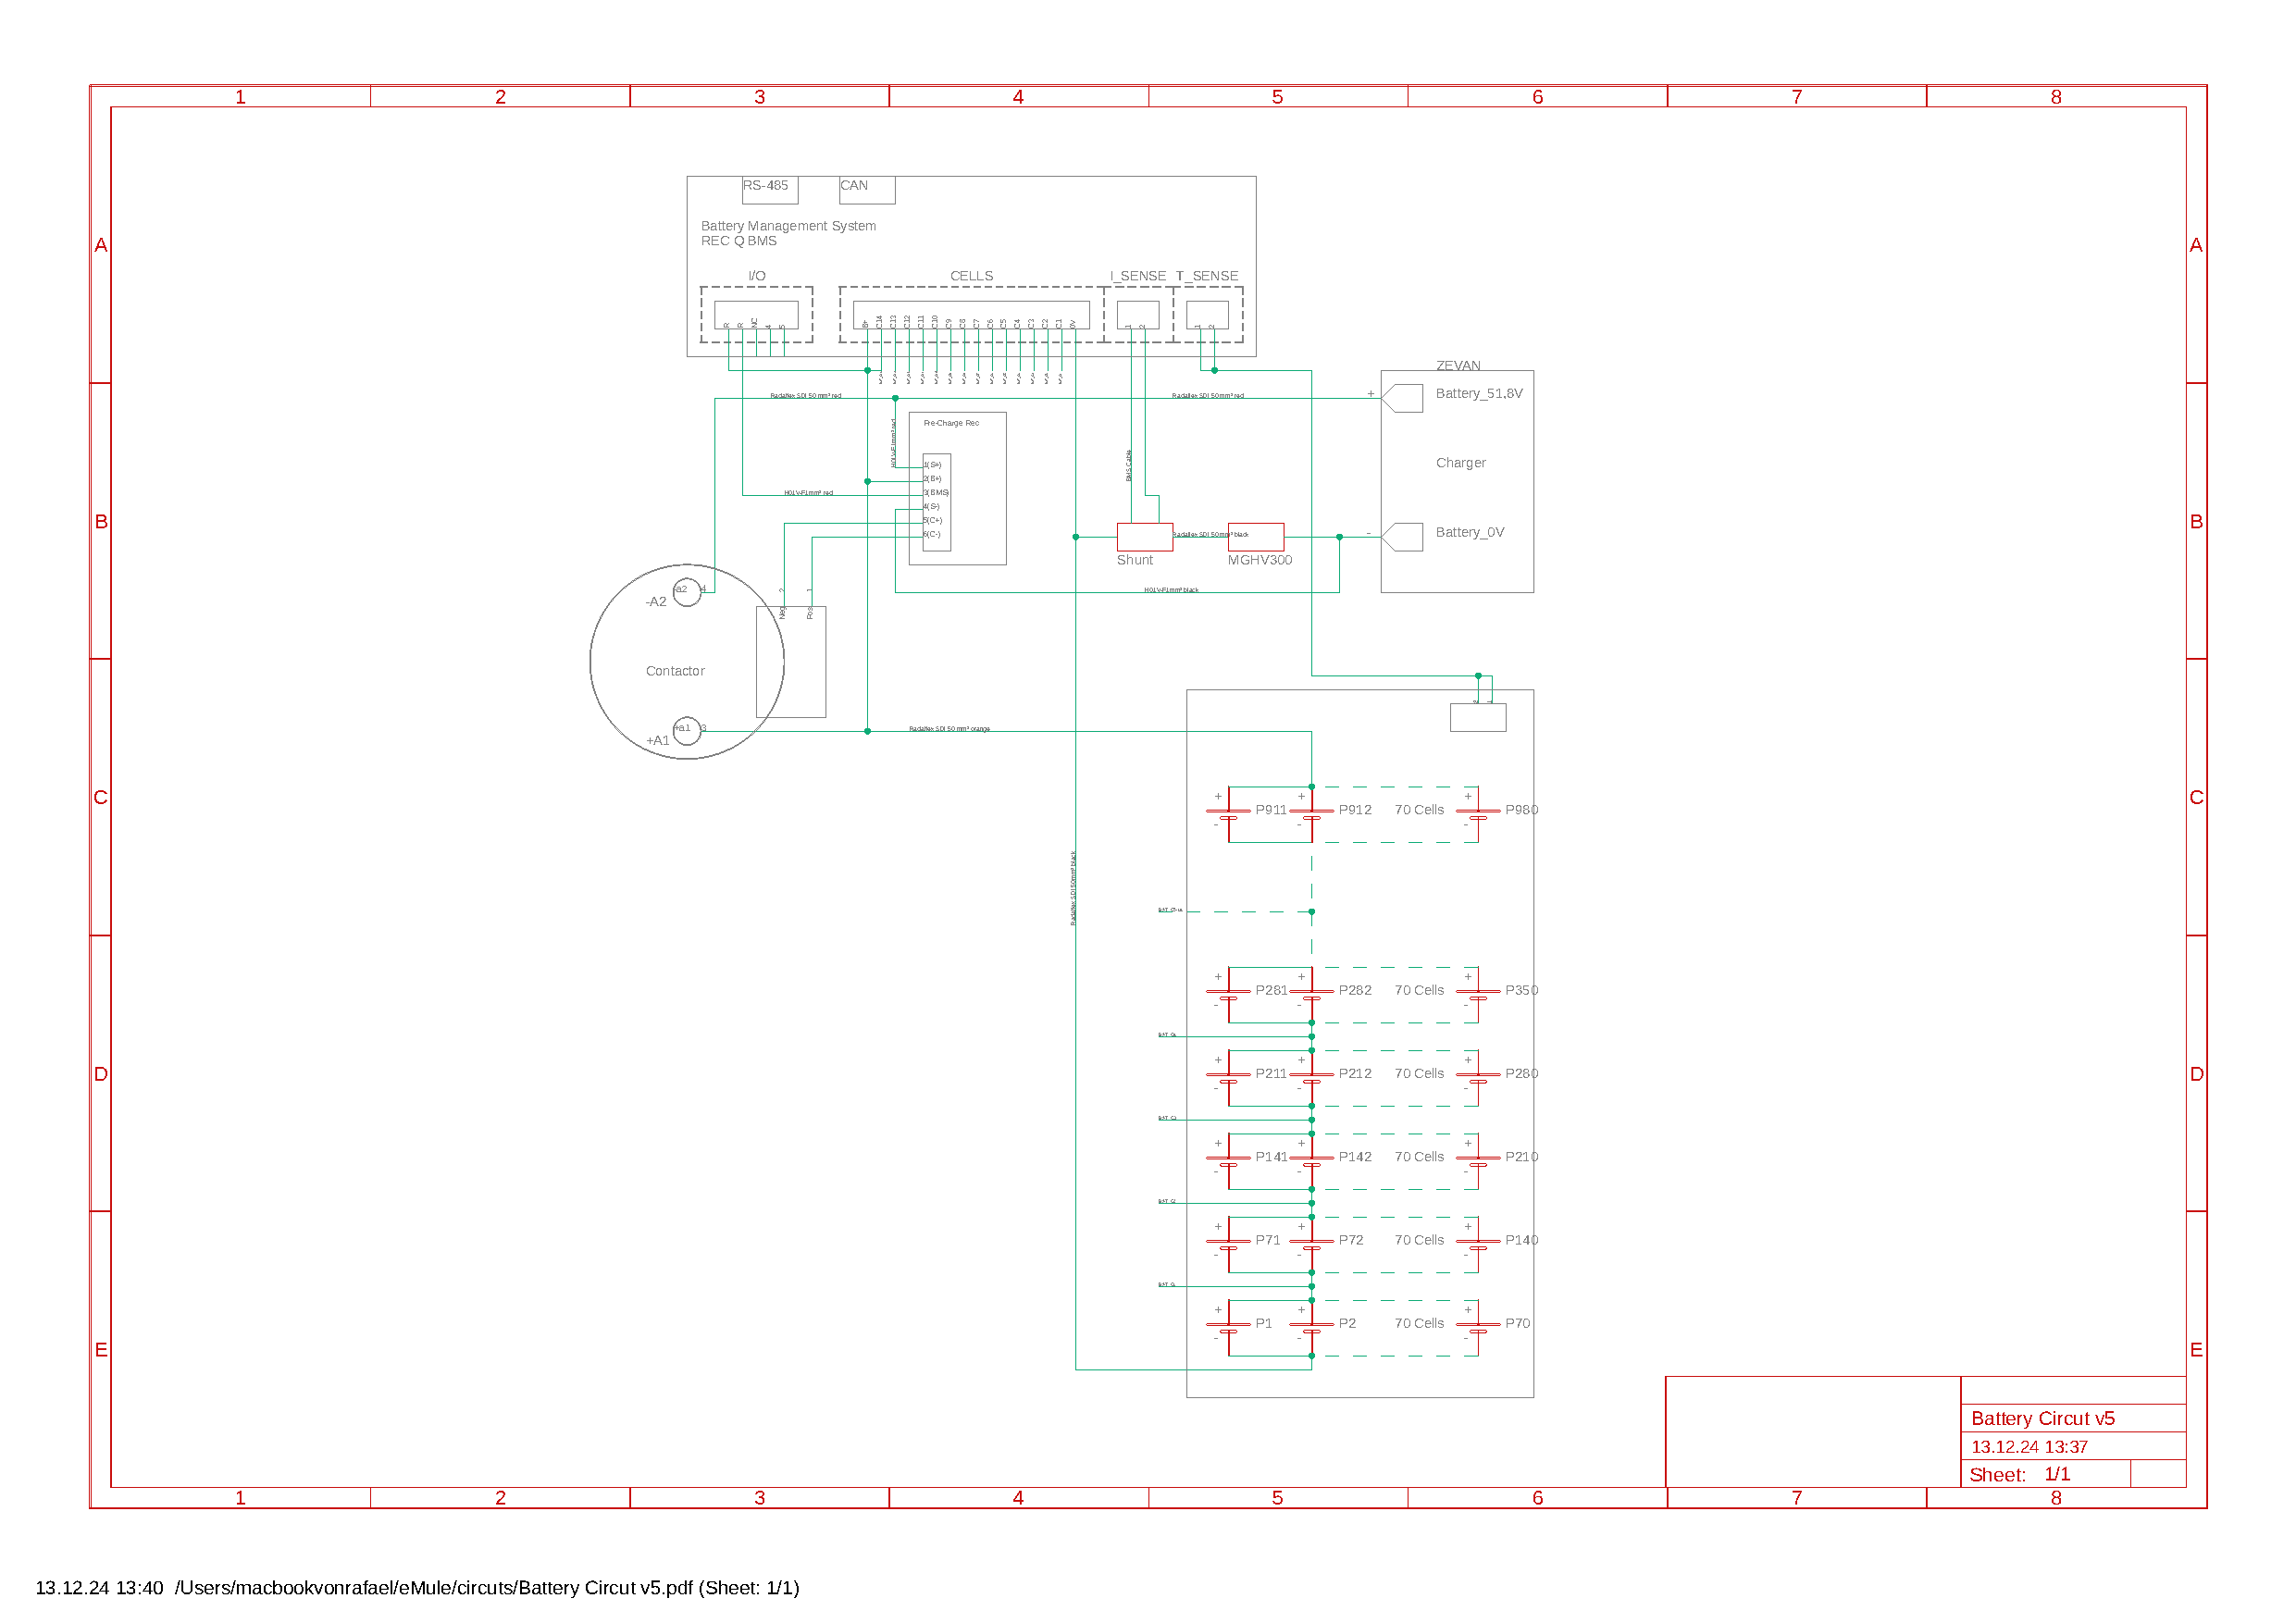
\includepdf[pages=1, trim=0cm 0cm 21cm 0cm, clip]{circuts/Battery Circut v5.pdf}

% Rechte Hälfte der A3-Seite
%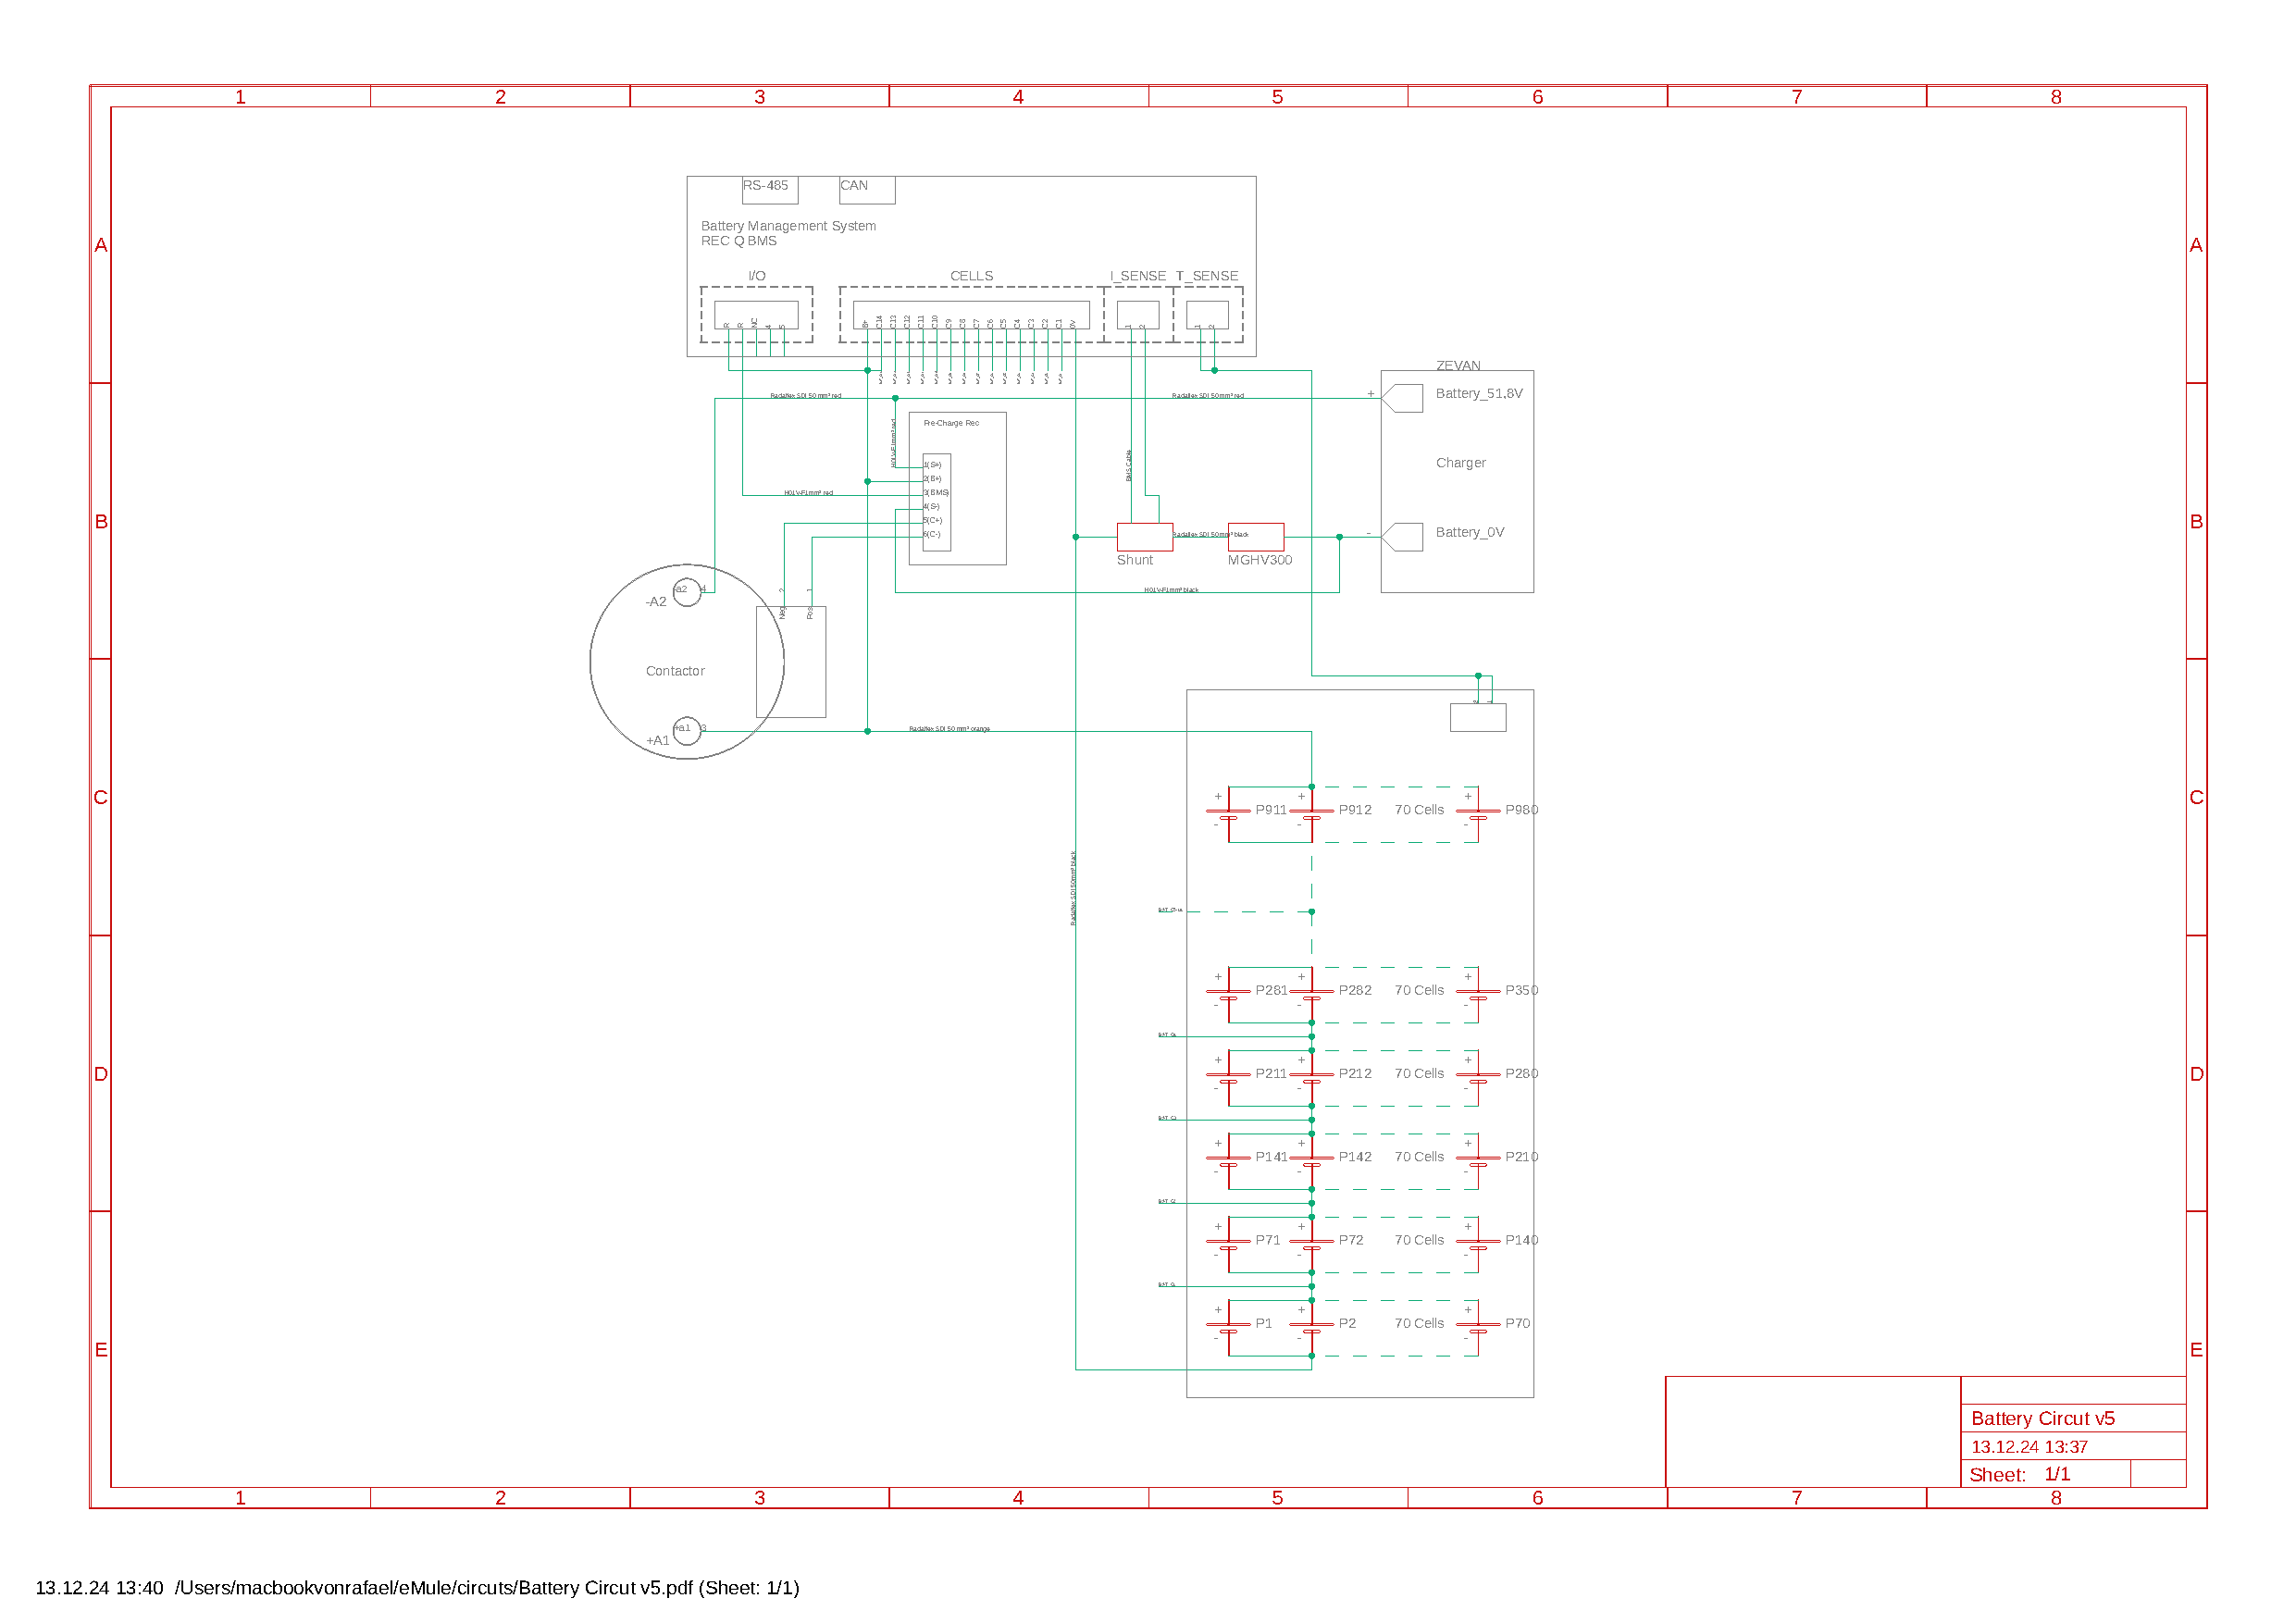
\includepdf[pages=1, trim=21cm 0cm 0cm 0cm, clip]{circuts/Battery Circut v5.pdf}

%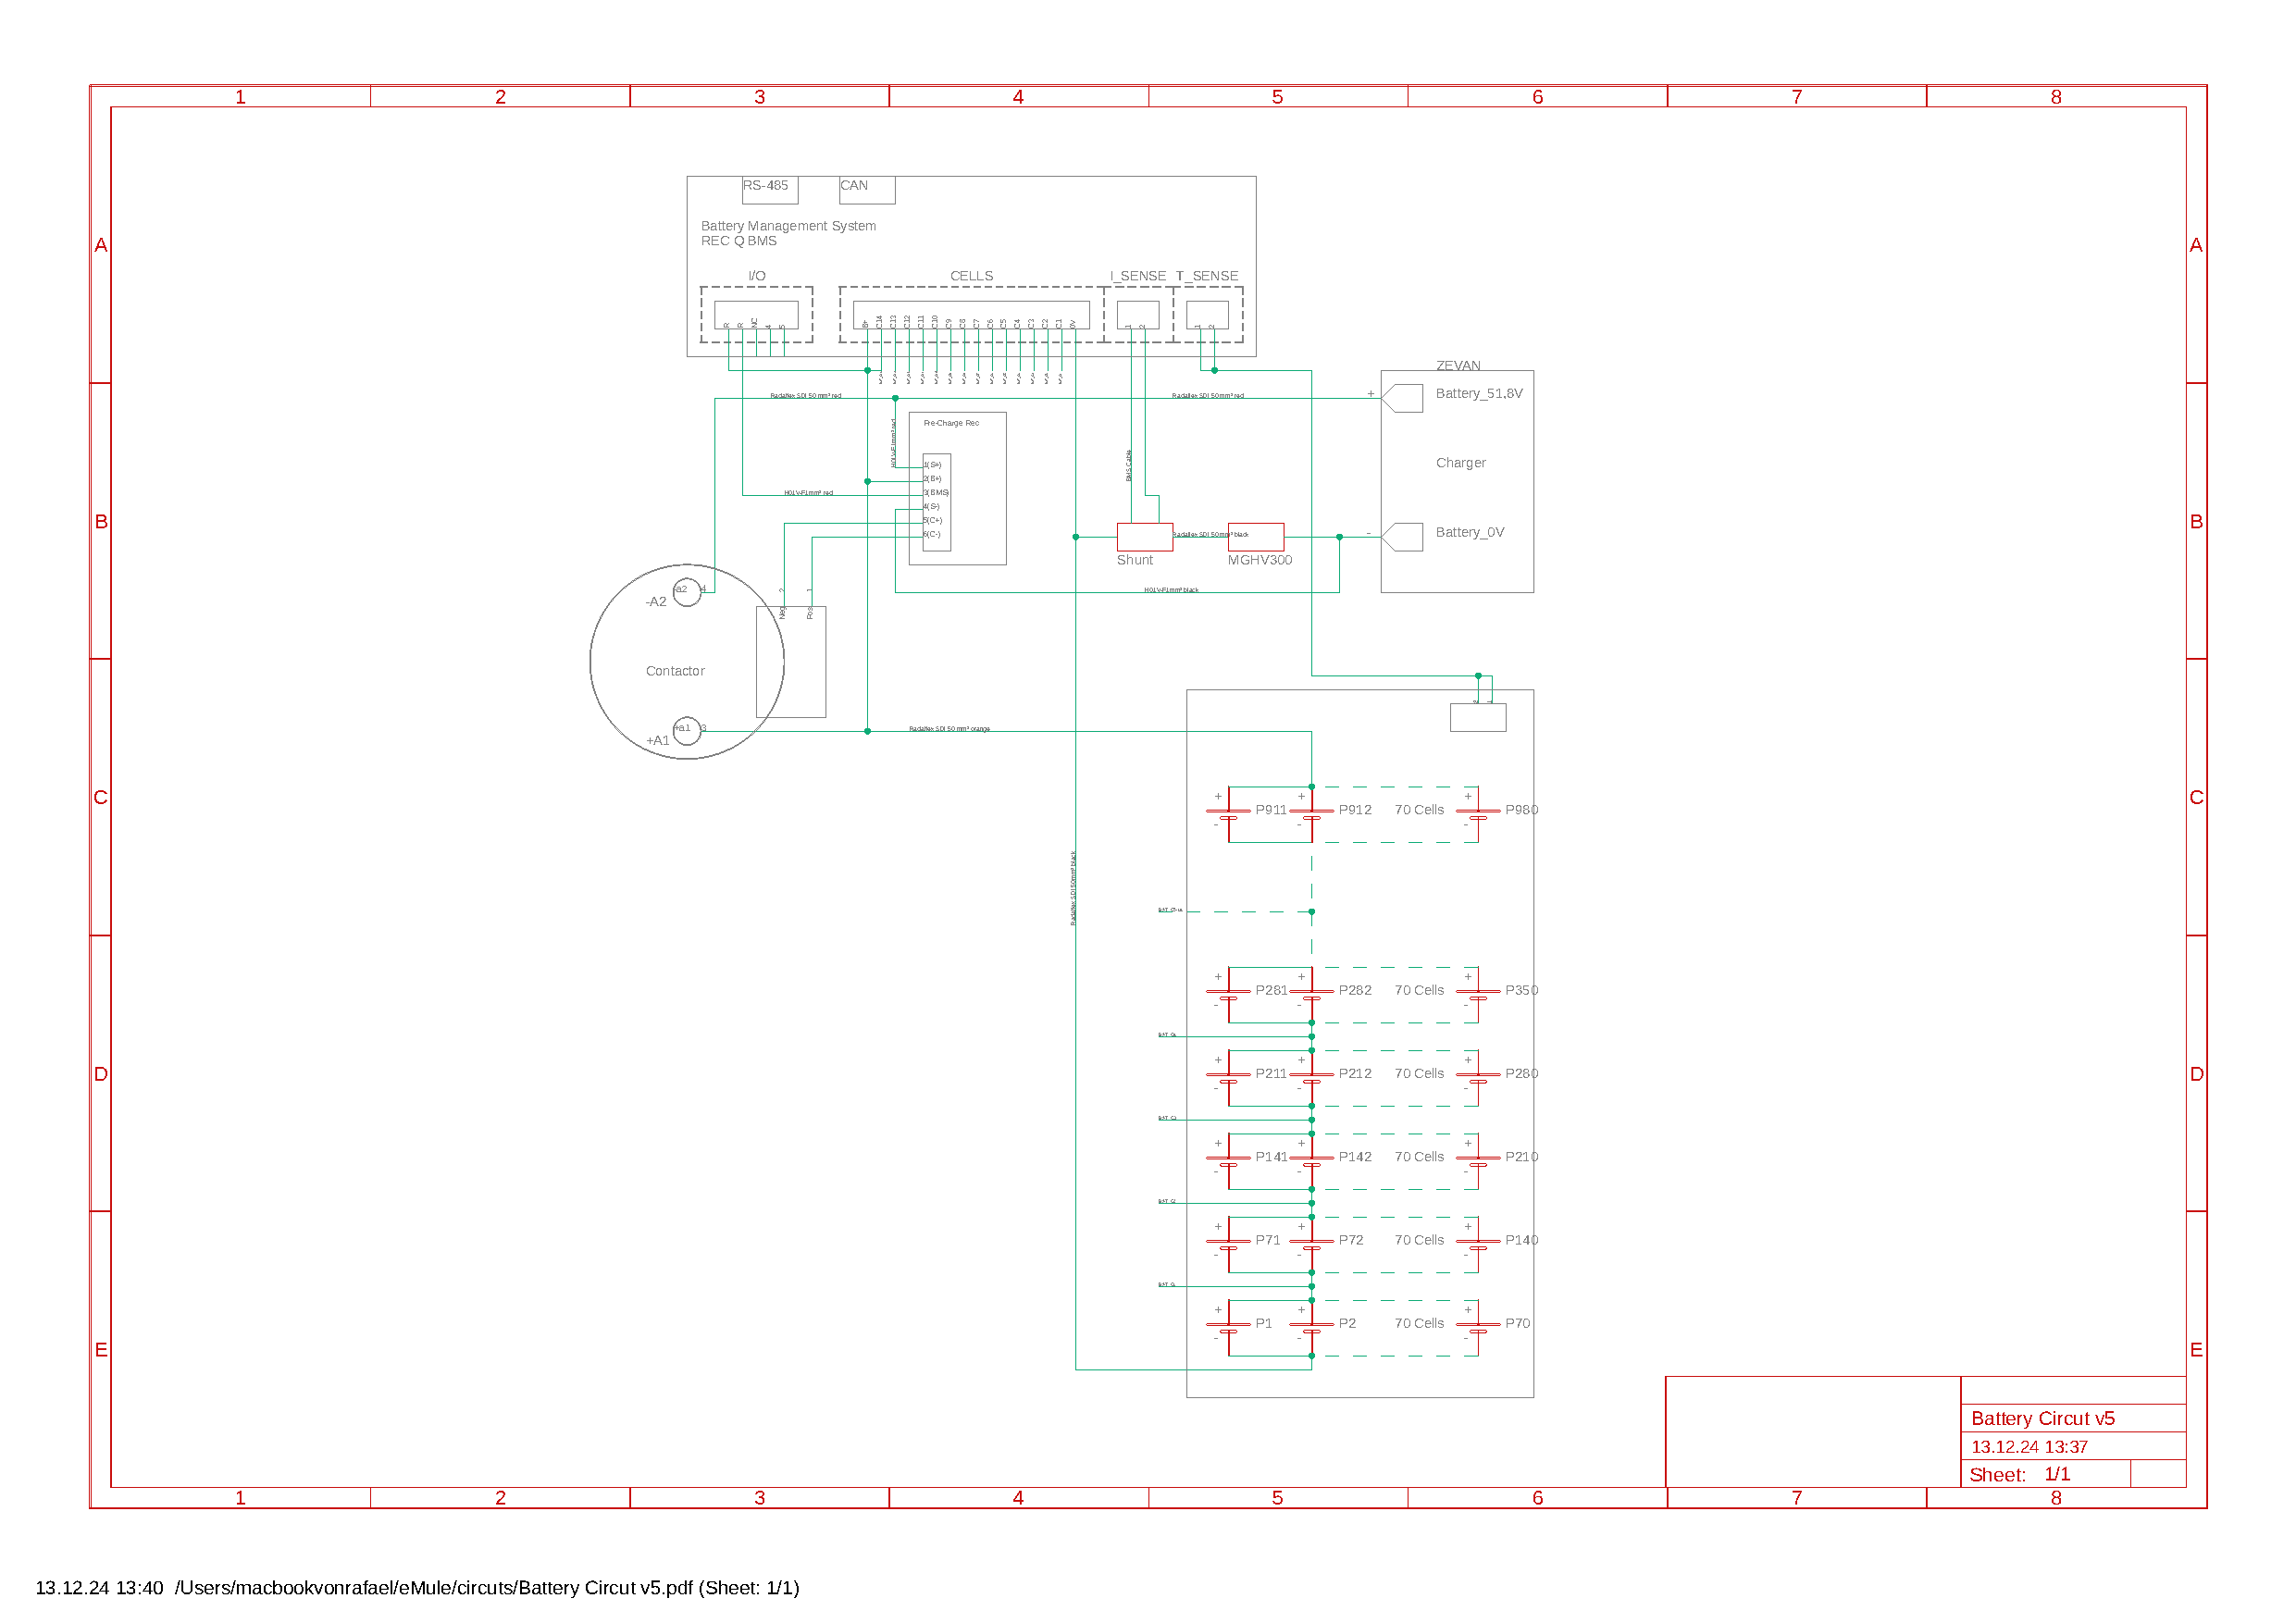
\includepdf[pages=1, angle=90, fitpaper=true]{circuts/Battery Circut v5.pdf}
\section{Circuit diagrams}
\subsection{Circuit diagram of the battery circuit}
%Für die Erstellung des \textit{Battery Circuit} (siehe Abbildung \ref{fig:battery_circuit}) Stromlaufplans nach festgelegter Norm und aktuellem Verbaustand wird der vorliegende Plan zunächst ausgedruckt. Im ersten Schritt wird dieser Stromlaufplan systematisch auf Unstimmigkeiten, wie fehlende Verbindungen oder unklare Symbolik, überprüft. Gefundene Fehler werden im nächsten Schritt markiert und anschließend korrigiert, wobei die Einhaltung elektrotechnischer Standards gewährleistet wird. Zudem erfolgt eine Layoutanpassung zur Verbesserung der Übersichtlichkeit. Im letzten Schritt muss herausgefunden werden, nach welcher Norm der Stromlaufplan erstellt wurde. Diese Norm muss recherchiert und in die von uns gewählte DIN EN 60617 Norm \glqq übersetzt\grqq {} werden. Der überarbeitete Stromlaufplan wird abschließend mit Autodesk Fusion 360 in ein DIN-A3-Format übertragen. Dabei werden Titelblock und Legende integriert, um die Professionalität und Lesbarkeit sicherzustellen.
In order to create the \textit{battery circuit} (see figure \ref{fig:battery_circuit}), the existing diagram is first printed out, and the circuit is then created in accordance with the defined standard and current installation status. In the initial phase, the circuit diagram is meticulously examined for any inconsistencies, including the absence of connections or the ambiguity of symbols. Any errors detected during this process are subsequently annotated in the subsequent stage, and then rectified, thus ensuring conformity with the relevant electrotechnical standards. The layout has been adapted to improve clarity. In the final step, it is necessary to determine the standard according to which the circuit diagram was created. It is imperative that this standard is thoroughly researched and \glqq translated\grqq {} into our chosen DIN EN 60617 standard. The revised circuit diagram is then transferred to a DIN A3 format using Autodesk Fusion 360. The integration of the title block and legend is paramount in ensuring the maintenance of a professional and legible appearance.

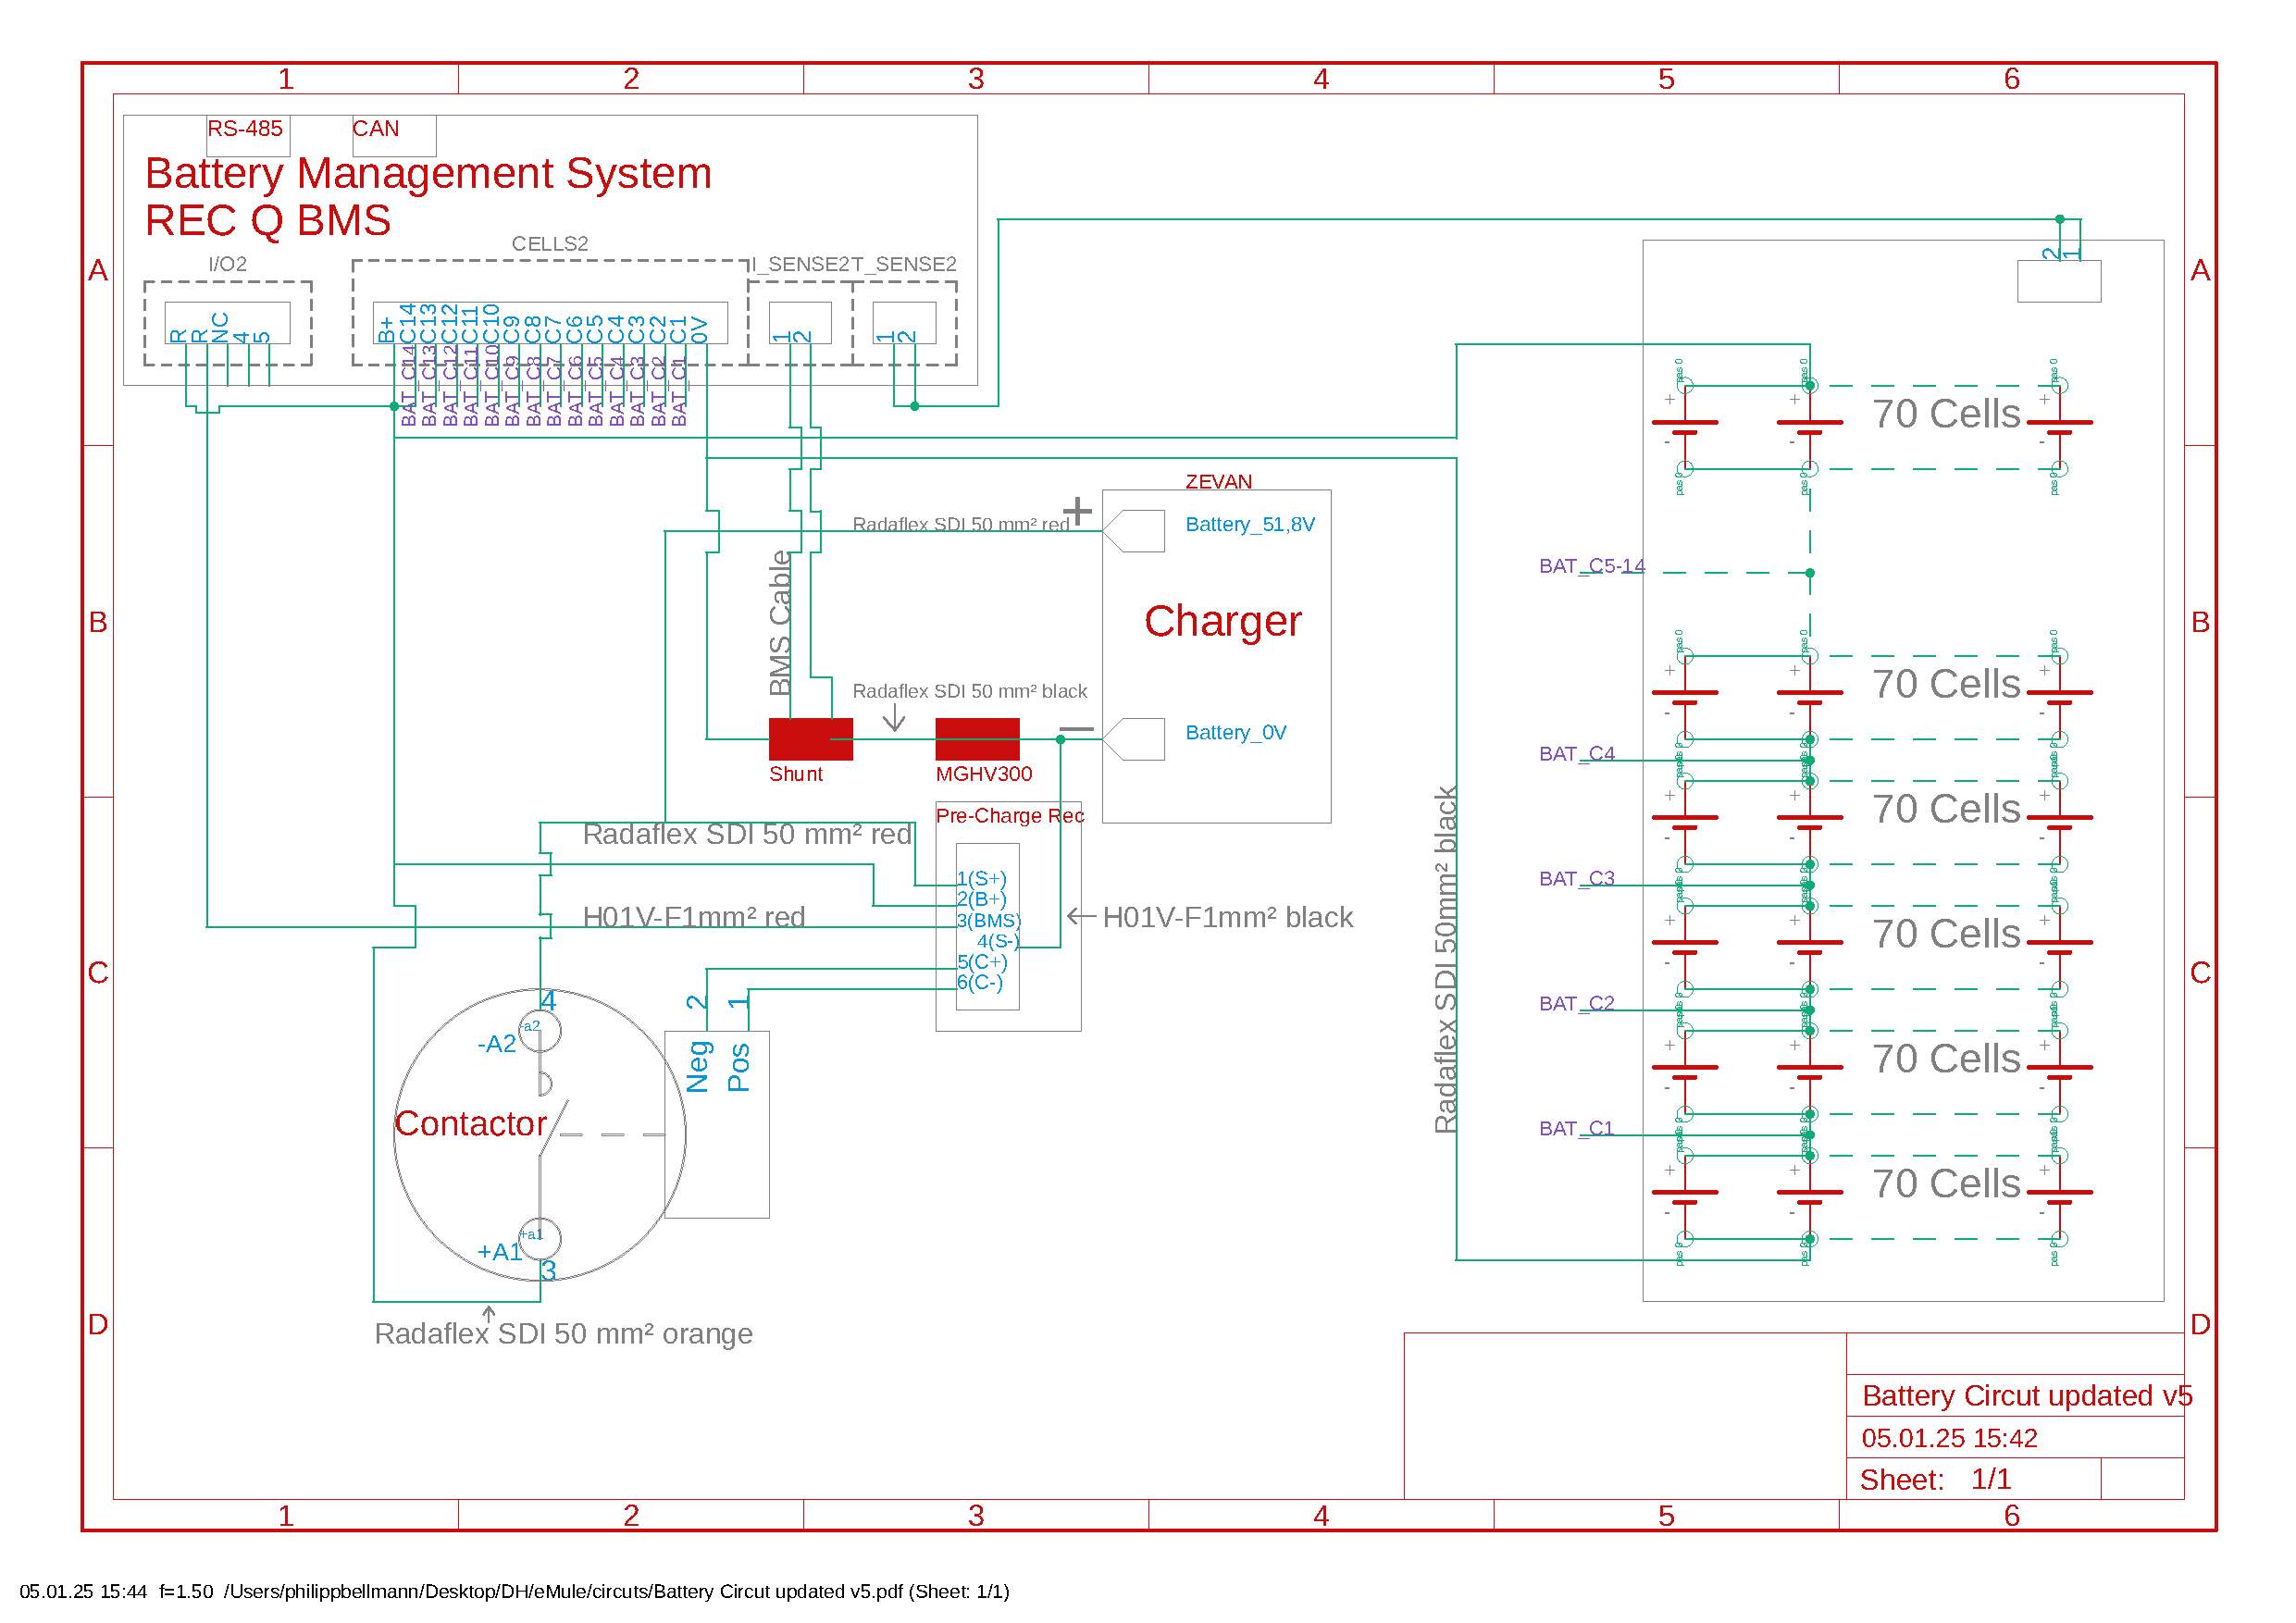
\includepdf[pages=1, fitpaper=true, pagecommand={%
	\thispagestyle{empty} % Entfernt Seitenzahlen und Kopfzeilen
	\begin{center}
		\vspace*{-5cm} % Verschiebt die Caption um 2 cm nach oben
		\hspace{10cm} % Verschiebt die Caption um 10 cm nach rechts
		\captionof{figure}{Circut diagram of the Battery Circuits} % Fügt die Caption ein
		\label{fig:battery_circuit} % Für Querverweise
	\end{center}
}]{circuts/Battery Circut updated.pdf}
\addtocounter{page}{1} % Seitenzähler korrekt erhöhen

% Zweite PDF: Motor Controller
\subsection{Circut diagram of the motor controller}
%Für die Erstellung des \textit{Motor Controller} (siehe Abbildung \ref{fig:motor_controller}) Stromlaufplans nach festgelegter Norm und aktuellem Verbaustand wird der vorliegende Plan zunächst ausgedruckt. Im ersten Schritt wird dieser Stromlaufplan systematisch auf Unstimmigkeiten, wie fehlende Verbindungen oder unklare Symbolik, überprüft. Gefundene Fehler werden im nächsten Schritt markiert und anschließend korrigiert, wobei die Einhaltung elektrotechnischer Standards gewährleistet wird. Zudem erfolgt eine Layoutanpassung zur Verbesserung der Übersichtlichkeit. Im letzten Schritt muss herausgefunden werden, nach welcher Norm der Stromlaufplan erstellt wurde. Diese Norm muss recherchiert und in die von uns gewählte DIN EN 60617 Norm \glqq übersetzt\grqq {} werden. Der überarbeitete Stromlaufplan wird abschließend mit Autodesk Fusion 360 in ein DIN-A3-Format übertragen. Dabei werden Titelblock und Legende integriert, um die Professionalität und Lesbarkeit sicherzustellen.

In order to create the \textit{motor controller} (see figure \ref{fig:motor_controller}) the existing diagram is first printed out, and the circuit is then created in accordance with the defined standard and current installation status. In the initial phase, the circuit diagram is meticulously examined for any inconsistencies, including the absence of connections or the ambiguity of symbols. Any errors detected during this process are subsequently annotated in the subsequent stage, and then rectified, thus ensuring conformity with the relevant electrotechnical standards. The layout has been adapted to improve clarity. In the final step, the standard according to which the circuit diagram was created must be determined. It is imperative that this standard is thoroughly researched and translated into the DIN EN 60617 standard selected by us. The revised circuit diagram is then transferred to a DIN A3 format using Autodesk Fusion 360. The integration of the title block and legend is a deliberate design choice that serves to enhance the document's professionalism and legibility.

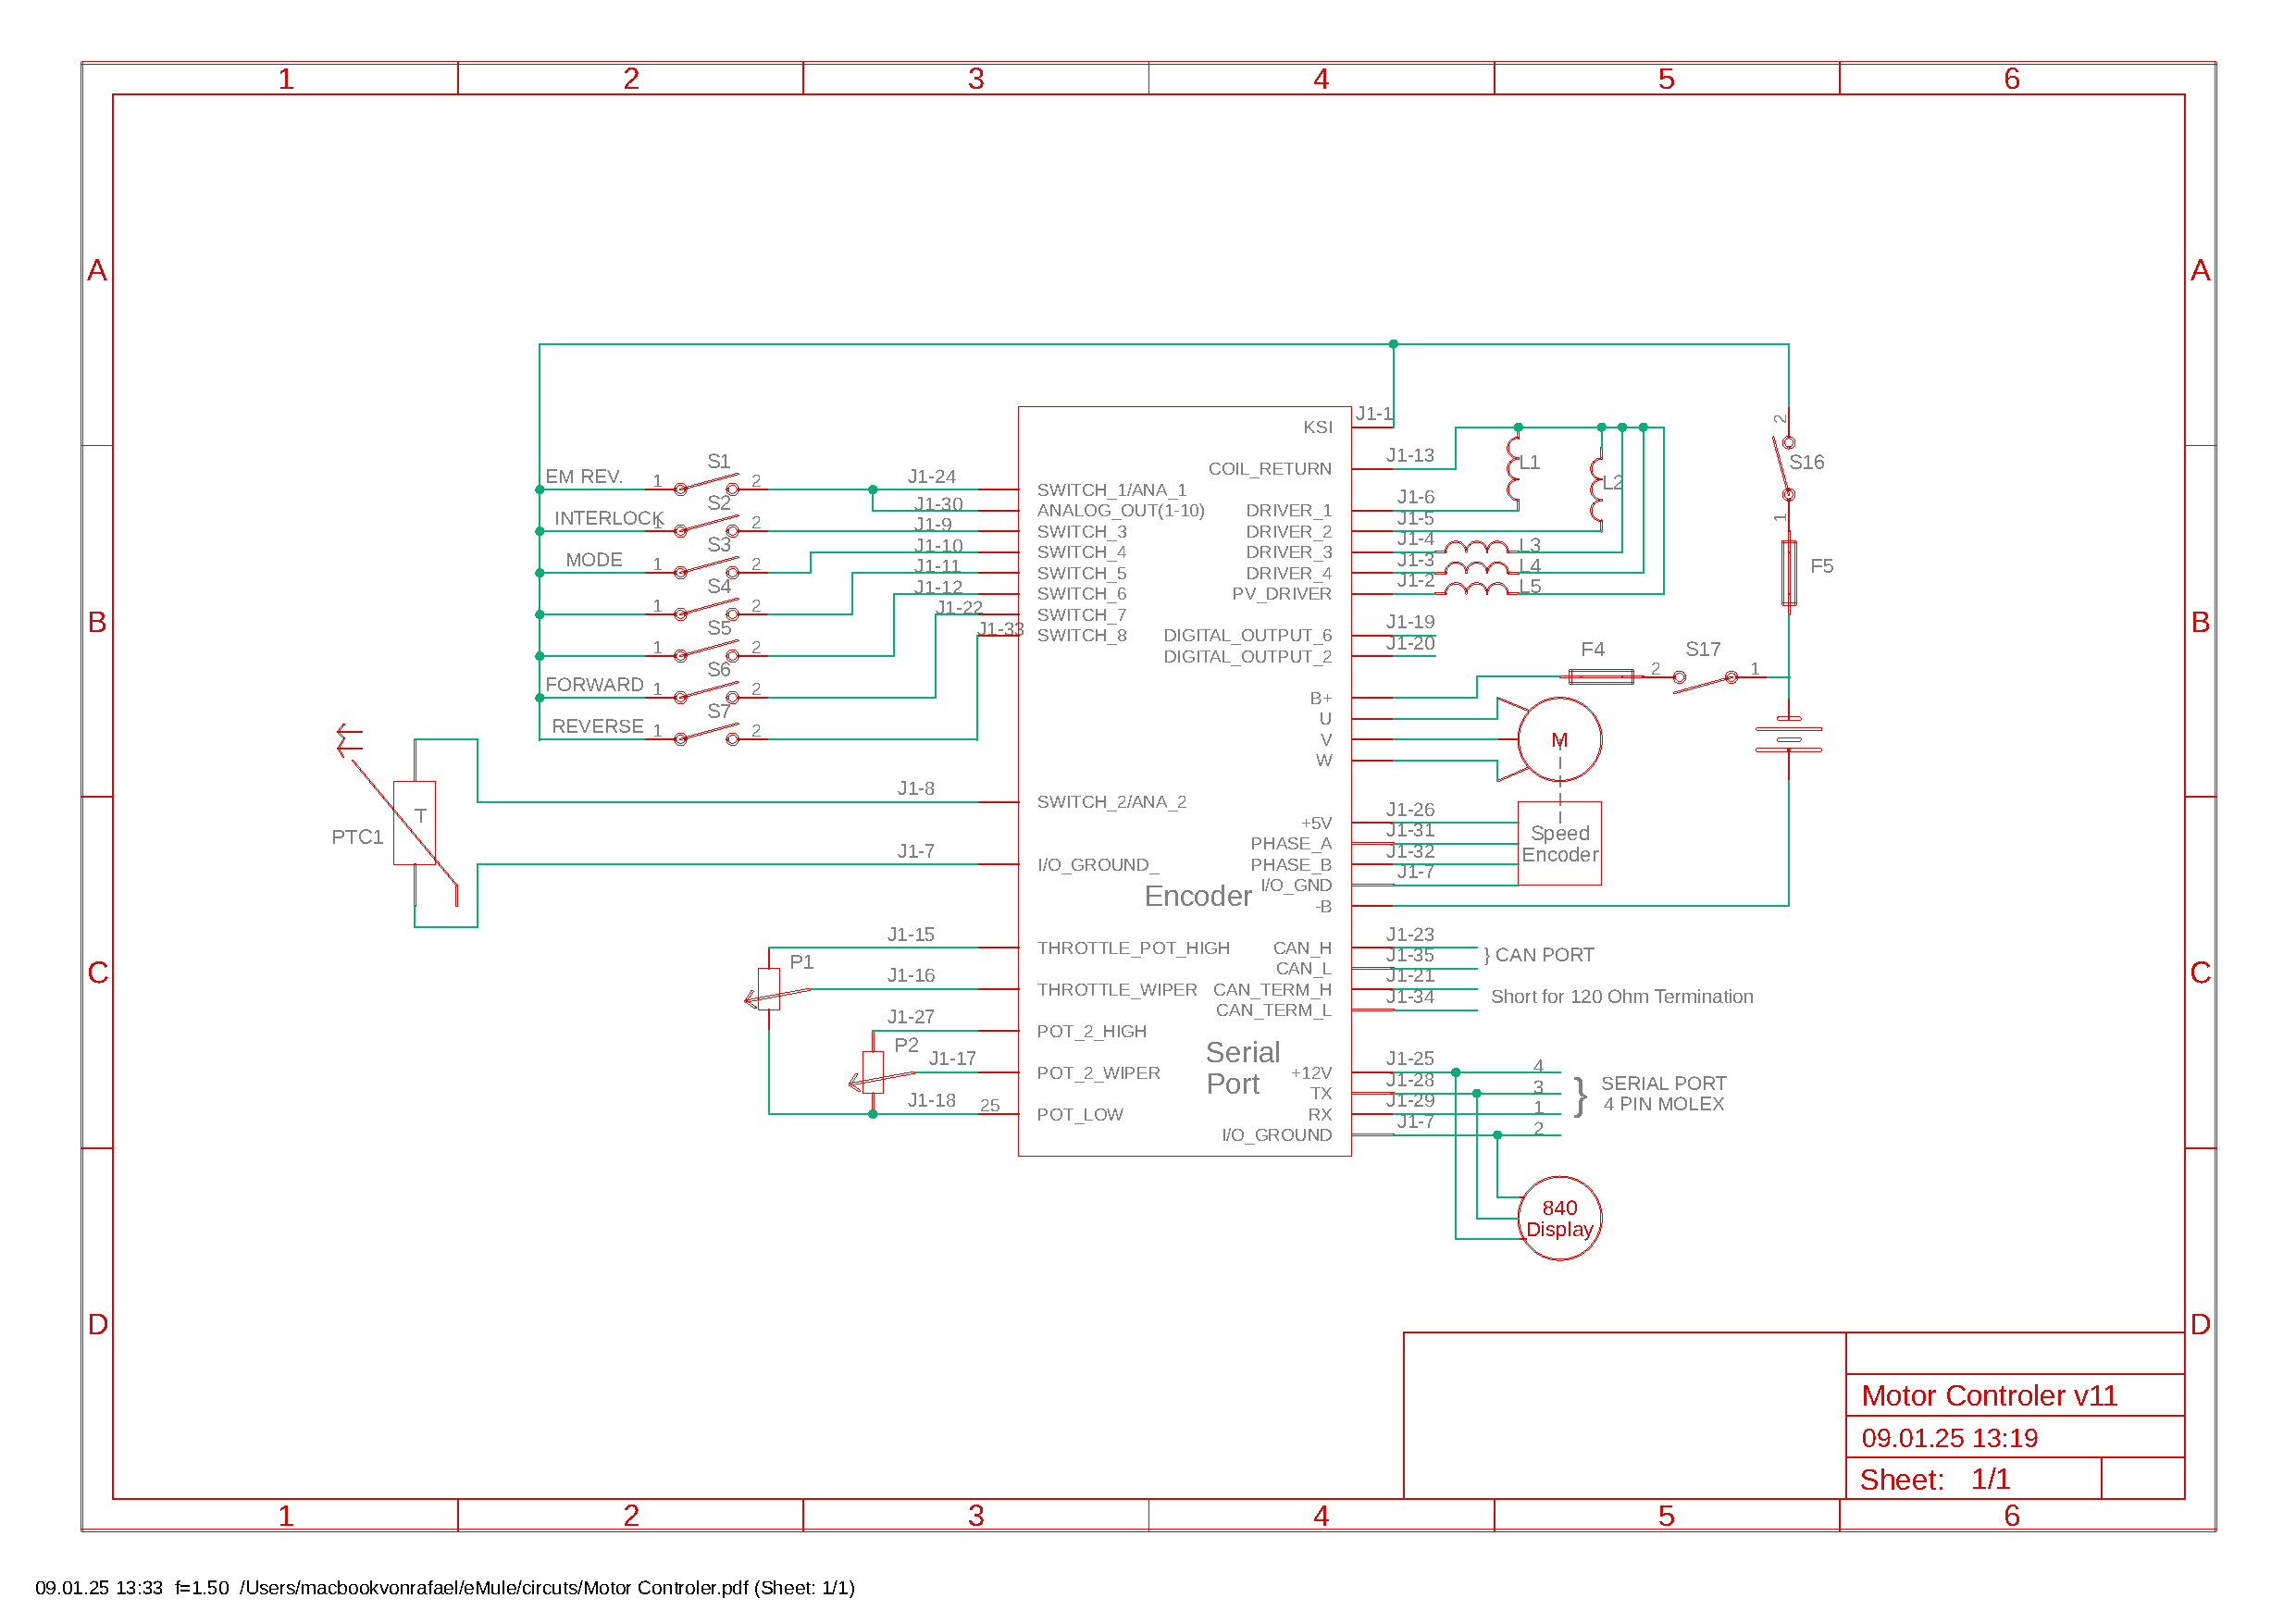
\includepdf[pages=1, fitpaper=true, pagecommand={%
	\thispagestyle{empty} % Entfernt Seitenzahlen und Kopfzeilen
	\begin{center}
		\captionof{figure}{Schaltplan des Motor Controllers} % Fügt die Caption ein
		\label{fig:motor_controller} % Für Querverweise
	\end{center}
}]{circuts/Motor Controler.pdf}
\addtocounter{page}{1} % Seitenzähler korrekt erhöhen

% Dritte PDF: LV-Onboard-Network
\subsection{Circut diagram of the LV onboard power supply}
%Für die Erstellung des \textit{LV-Onboard-Netz} (siehe Abbildung \ref{fig:lv_onboard_network}) Stromlaufplans nach festgelegter Norm und aktuellem Verbaustand wird der vorliegende Plan zunächst ausgedruckt. Im ersten Schritt wird dieser Stromlaufplan systematisch auf Unstimmigkeiten, wie fehlende Verbindungen oder unklare Symbolik, überprüft. Gefundene Fehler werden im nächsten Schritt markiert und anschließend korrigiert, wobei die Einhaltung elektrotechnischer Standards gewährleistet wird. Zudem erfolgt eine Layoutanpassung zur Verbesserung der Übersichtlichkeit. Im letzten Schritt muss herausgefunden werden, nach welcher Norm der Stromlaufplan erstellt wurde. Diese Norm muss recherchiert und in die von uns gewählte DIN EN 60617 Norm \glqq übersetzt\grqq {} werden. Der überarbeitete Stromlaufplan wird abschließend mit Autodesk Fusion 360 in ein DIN-A3-Format übertragen. Dabei werden Titelblock und Legende integriert, um die Professionalität und Lesbarkeit sicherzustellen.

In order to establish the LV onboard power supply (see figure \ref{fig:lv_onboard_network}), the circuit diagram must be created in accordance with the defined standard and current installation status. To this end, the existing diagram is to be printed out. In the initial phase, the circuit diagram is meticulously examined for any inconsistencies, including the absence of connections or the ambiguity of symbols. Any errors detected during this process are subsequently annotated in the subsequent stage, and then rectified, thus ensuring conformity with the relevant electrotechnical standards. The layout has been adapted to improve clarity. In the final step, the standard according to which the circuit diagram was created must be determined. It is imperative that this standard is thoroughly researched and translated into the DIN EN 60617 standard, which has been selected by us. The revised circuit diagram is then transferred to a DIN A3 format using Autodesk Fusion 360. The integration of the title block and legend is a deliberate design choice that serves to enhance the document's professionalism and legibility.


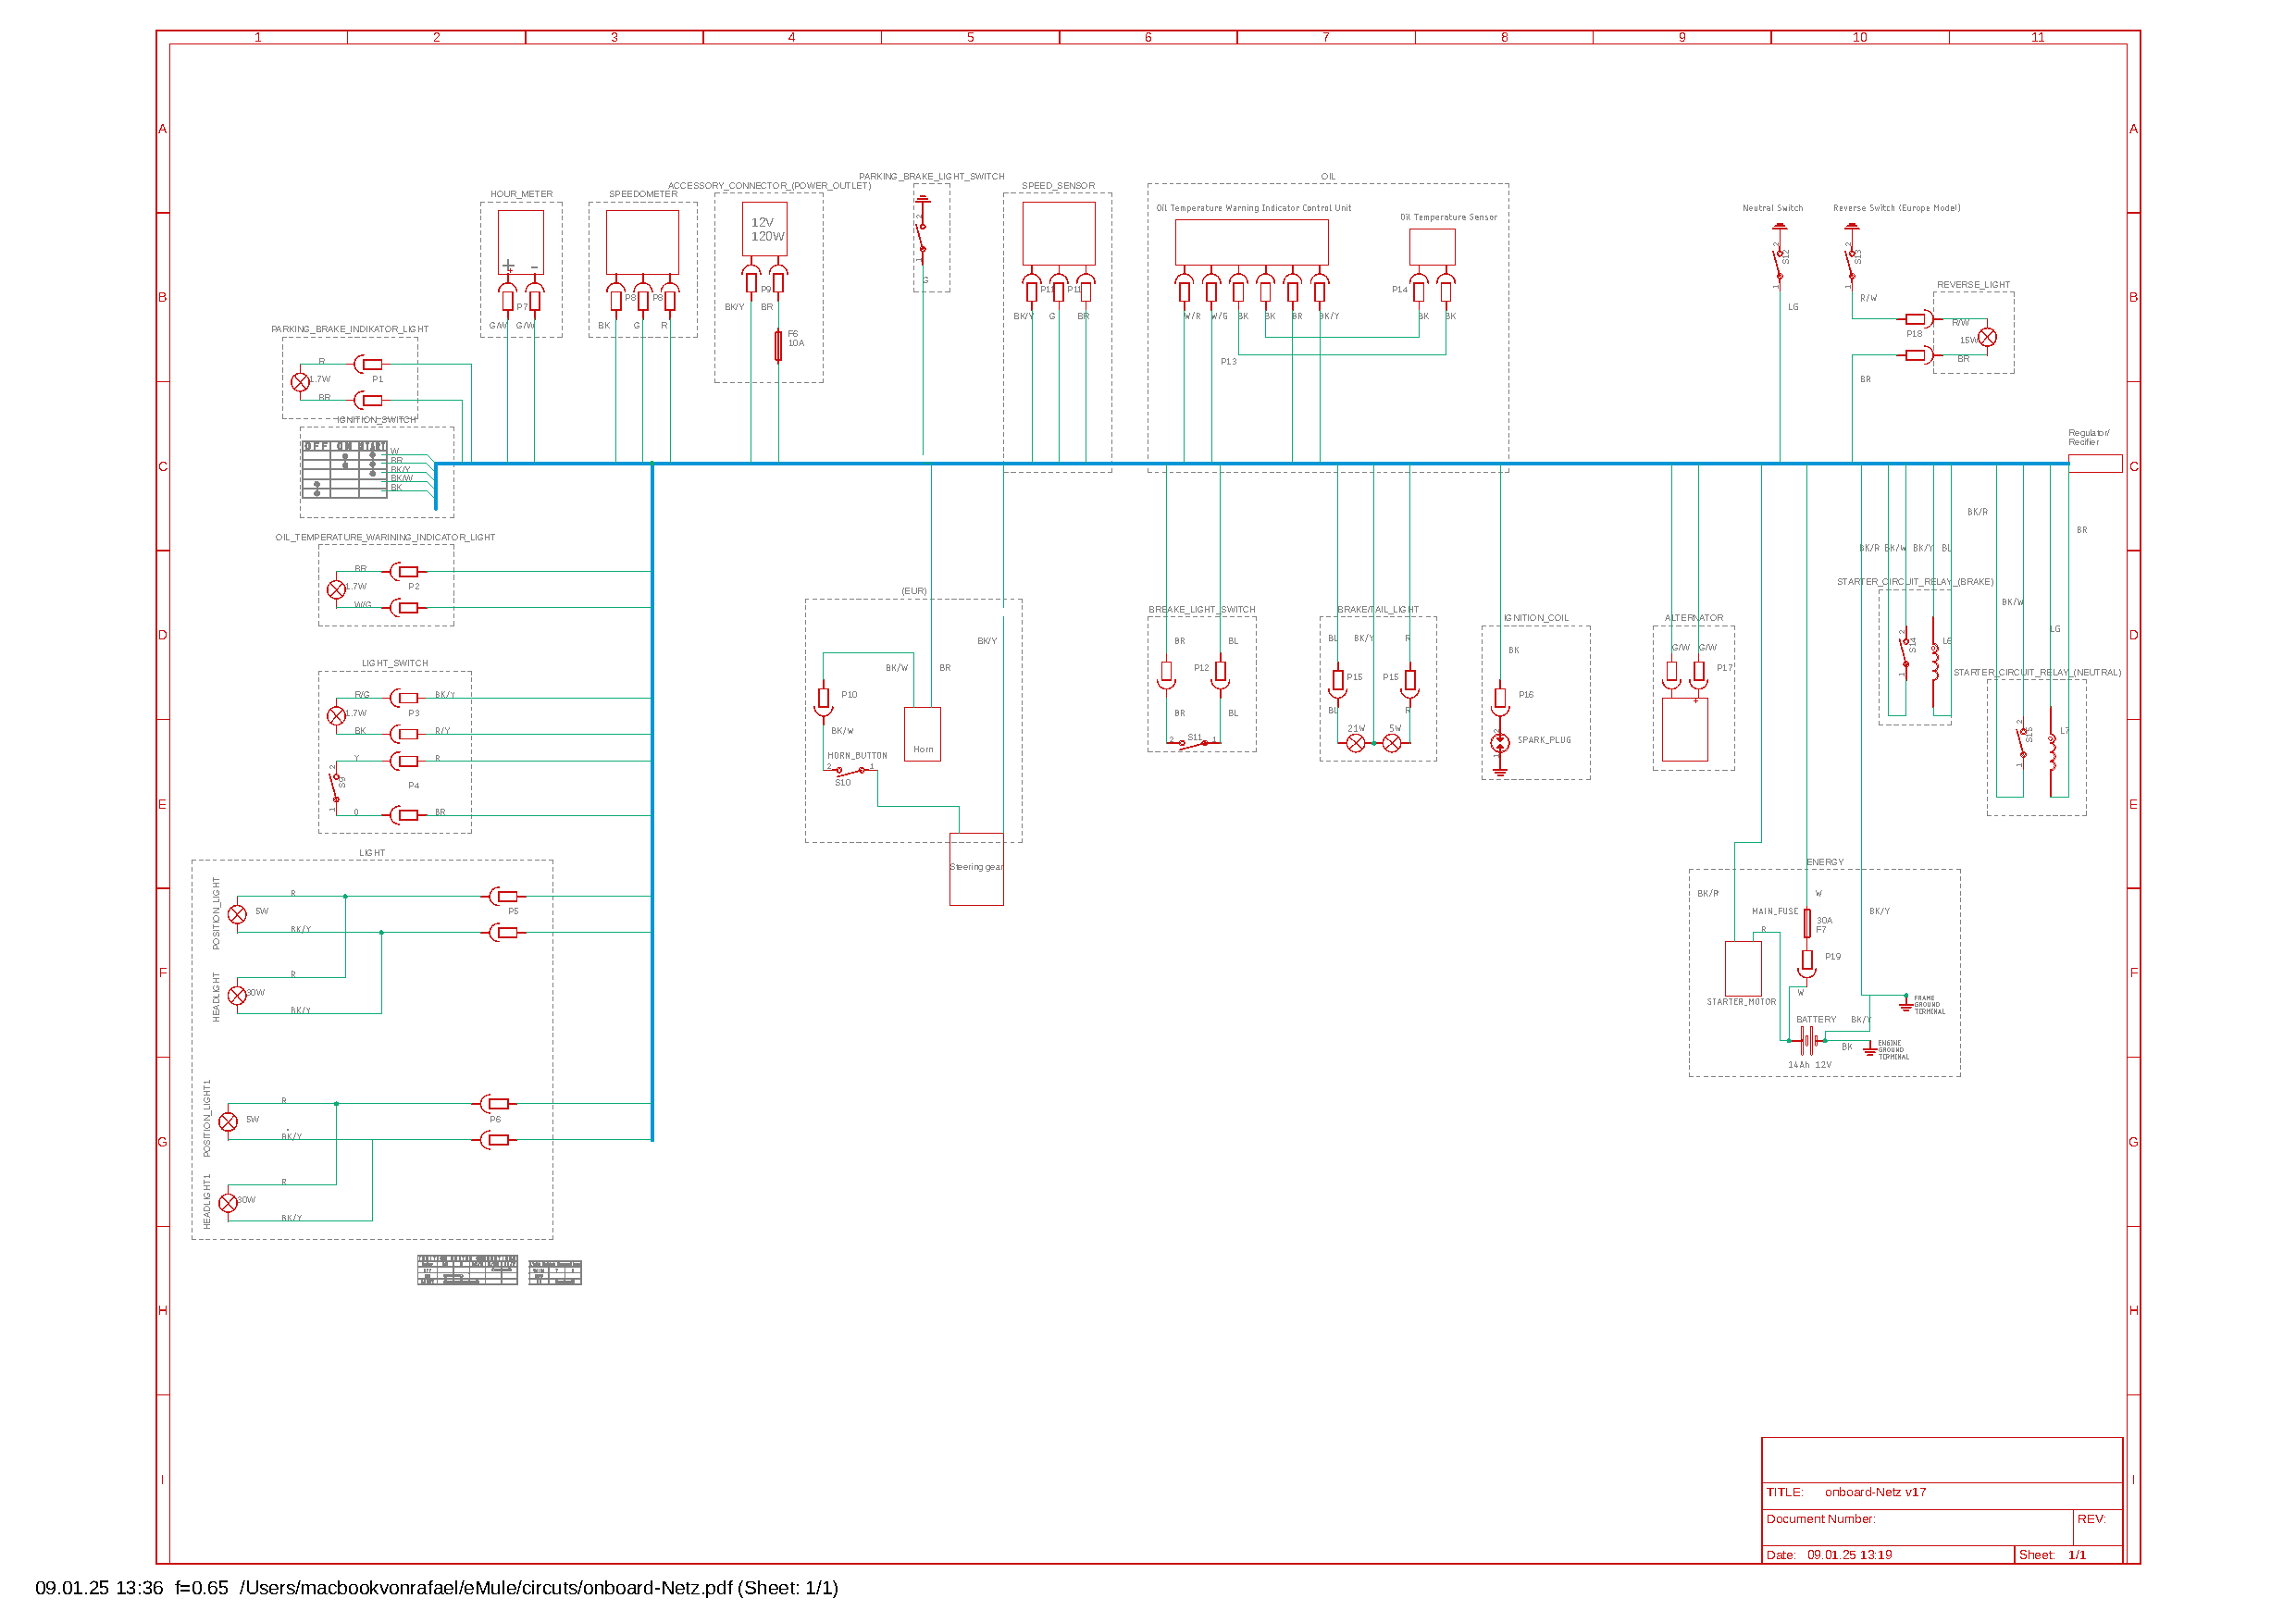
\includepdf[pages=1, fitpaper=true, pagecommand={%
	\thispagestyle{empty} % Entfernt Seitenzahlen und Kopfzeilen
	\begin{center}
		\vspace*{-2cm} % Verschiebt die Caption um 2 cm nach oben
		\captionof{figure}{Circut diagram of the LV onboard power supply} % Fügt die Caption ein
		\label{fig:lv_onboard_network} % Für Querverweise
	\end{center}
}]{circuts/onboard-Netz.pdf}
\addtocounter{page}{1} % Seitenzähler korrekt erhöhen

% Vierte PDF: Charger Temperature Control
\subsection{Circut diagram of the charger temperature control}
%Für die Erstellung des \textit{charger temperature control} (siehe Abbildung \ref{fig:charger_temperature_control}) Stromlaufplans nach festgelegter Norm und aktuellem Verbaustand wird zunächst eine händische Skizze des Systems, durch die für den Einbau zuständigen Kollegen, angefertigt und an das Dokumentationsteam weitergegeben. Im ersten Schritt wird dieser Stromlaufplan systematisch auf Unstimmigkeiten, wie fehlende Verbindungen oder unklare Symbolik, überprüft. Gefundene Fehler werden im nächsten Schritt markiert und anschließend korrigiert, wobei die Einhaltung elektrotechnischer Standards gewährleistet wird. Zudem erfolgt eine Layoutanpassung zur Verbesserung der Übersichtlichkeit. Im letzten Schritt muss die Normkonformität der Stromlaufplanskizze überprüft werden. Der überarbeitete Stromlaufplan wird abschließend mit Autodesk Fusion 360 in ein DIN-A3-Format übertragen. Dabei werden Titelblock und Legende integriert, um die Professionalität und Lesbarkeit sicherzustellen.

In order to create the circuit diagram for the charger temperature control (see Figure \ref{fig:charger_temperature_control}), it is first necessary to create a manual sketch of the system. This is to be done according to the defined standard and current installation status. The creation of the manual sketch is the responsibility of the colleagues who are responsible for installation. It is then necessary to pass the sketch to the documentation team. In the initial phase, the circuit diagram is meticulously examined for any potential discrepancies, including the absence of connections or the ambiguity of symbols. Any errors detected during this process are subsequently annotated in the subsequent stage, and then rectified, thus ensuring conformity with the relevant electrotechnical standards. The layout has been adapted to improve clarity. In the final step of the process, the conformity of the circuit diagram with the relevant standards must be checked. The revised circuit diagram is then transferred to a DIN A3 format using Autodesk Fusion 360. The integration of the title block and legend is a deliberate design choice that serves to enhance the document's professionalism and legibility.
\textbf{\textit{\underline{!!!!!!!Einfügen @Buck}}}
%!!!!! Funktioniert bei Phibo nicht!!!!

%\includepdf[pages=1, fitpaper=true, pagecommand={%
%	\thispagestyle{empty} % Entfernt Seitenzahlen und Kopfzeilen
%	\begin{center}
%		\captionof{figure}{Schaltplan der Charger Temperature Control} % Fügt die Caption ein
%		\label{fig:charger_temperature_control} % Für Querverweise
%	\end{center}
% }]{circuts/Temperatursteuerung des Ladegerätes.pdf}
%\addtocounter{page}{1} % Seitenzähler korrekt erhöhen

% Fünfte PDF: HV-Onboard-Network
\subsection{Circut diagram of the HV onboard power supply}
%Für die Erstellung des \textit{HV-Onboard-Network} (siehe Abbildung \ref{fig:hv_onboard_network}) Stromlaufplans nach festgelegter Norm und aktuellem Verbaustand wird zunächst eine händische Skizze des Systems, durch die für den Einbau zuständigen Kollegen, angefertigt und an das Dokumentationsteam weitergegeben. Im ersten Schritt wird dieser Stromlaufplan systematisch auf Unstimmigkeiten, wie fehlende Verbindungen oder unklare Symbolik, überprüft. Gefundene Fehler werden im nächsten Schritt markiert und anschließend korrigiert, wobei die Einhaltung elektrotechnischer Standards gewährleistet wird. Zudem erfolgt eine Layoutanpassung zur Verbesserung der Übersichtlichkeit. Im letzten Schritt muss die Normkonformität der Stromlaufplanskizze überprüft werden. Der überarbeitete Stromlaufplan wird abschließend mit Autodesk Fusion 360 in ein DIN-A3-Format übertragen. Dabei werden Titelblock und Legende integriert, um die Professionalität und Lesbarkeit sicherzustellen.

The creation of the HV onboard power supply (see Figure \ref{fig:hv_onboard_network}) is to be undertaken in accordance with the defined standard and current installation status. To this end, a manual sketch of the system is to be made by the installation team and subsequently passed to the documentation team. In the initial phase, the circuit diagram is meticulously examined for any potential discrepancies, including the absence of connections or the ambiguity of symbols. Any errors detected during this process are subsequently annotated in the subsequent stage, and then rectified, thus ensuring conformity with the relevant electrotechnical standards. The layout has been adapted to improve clarity. In the final step of the process, the conformity of the circuit diagram with the relevant standards must be checked. The revised circuit diagram is then transferred to a DIN A3 format using Autodesk Fusion 360. The integration of the title block and legend is a deliberate design choice that serves to enhance the document's professionalism and legibility.

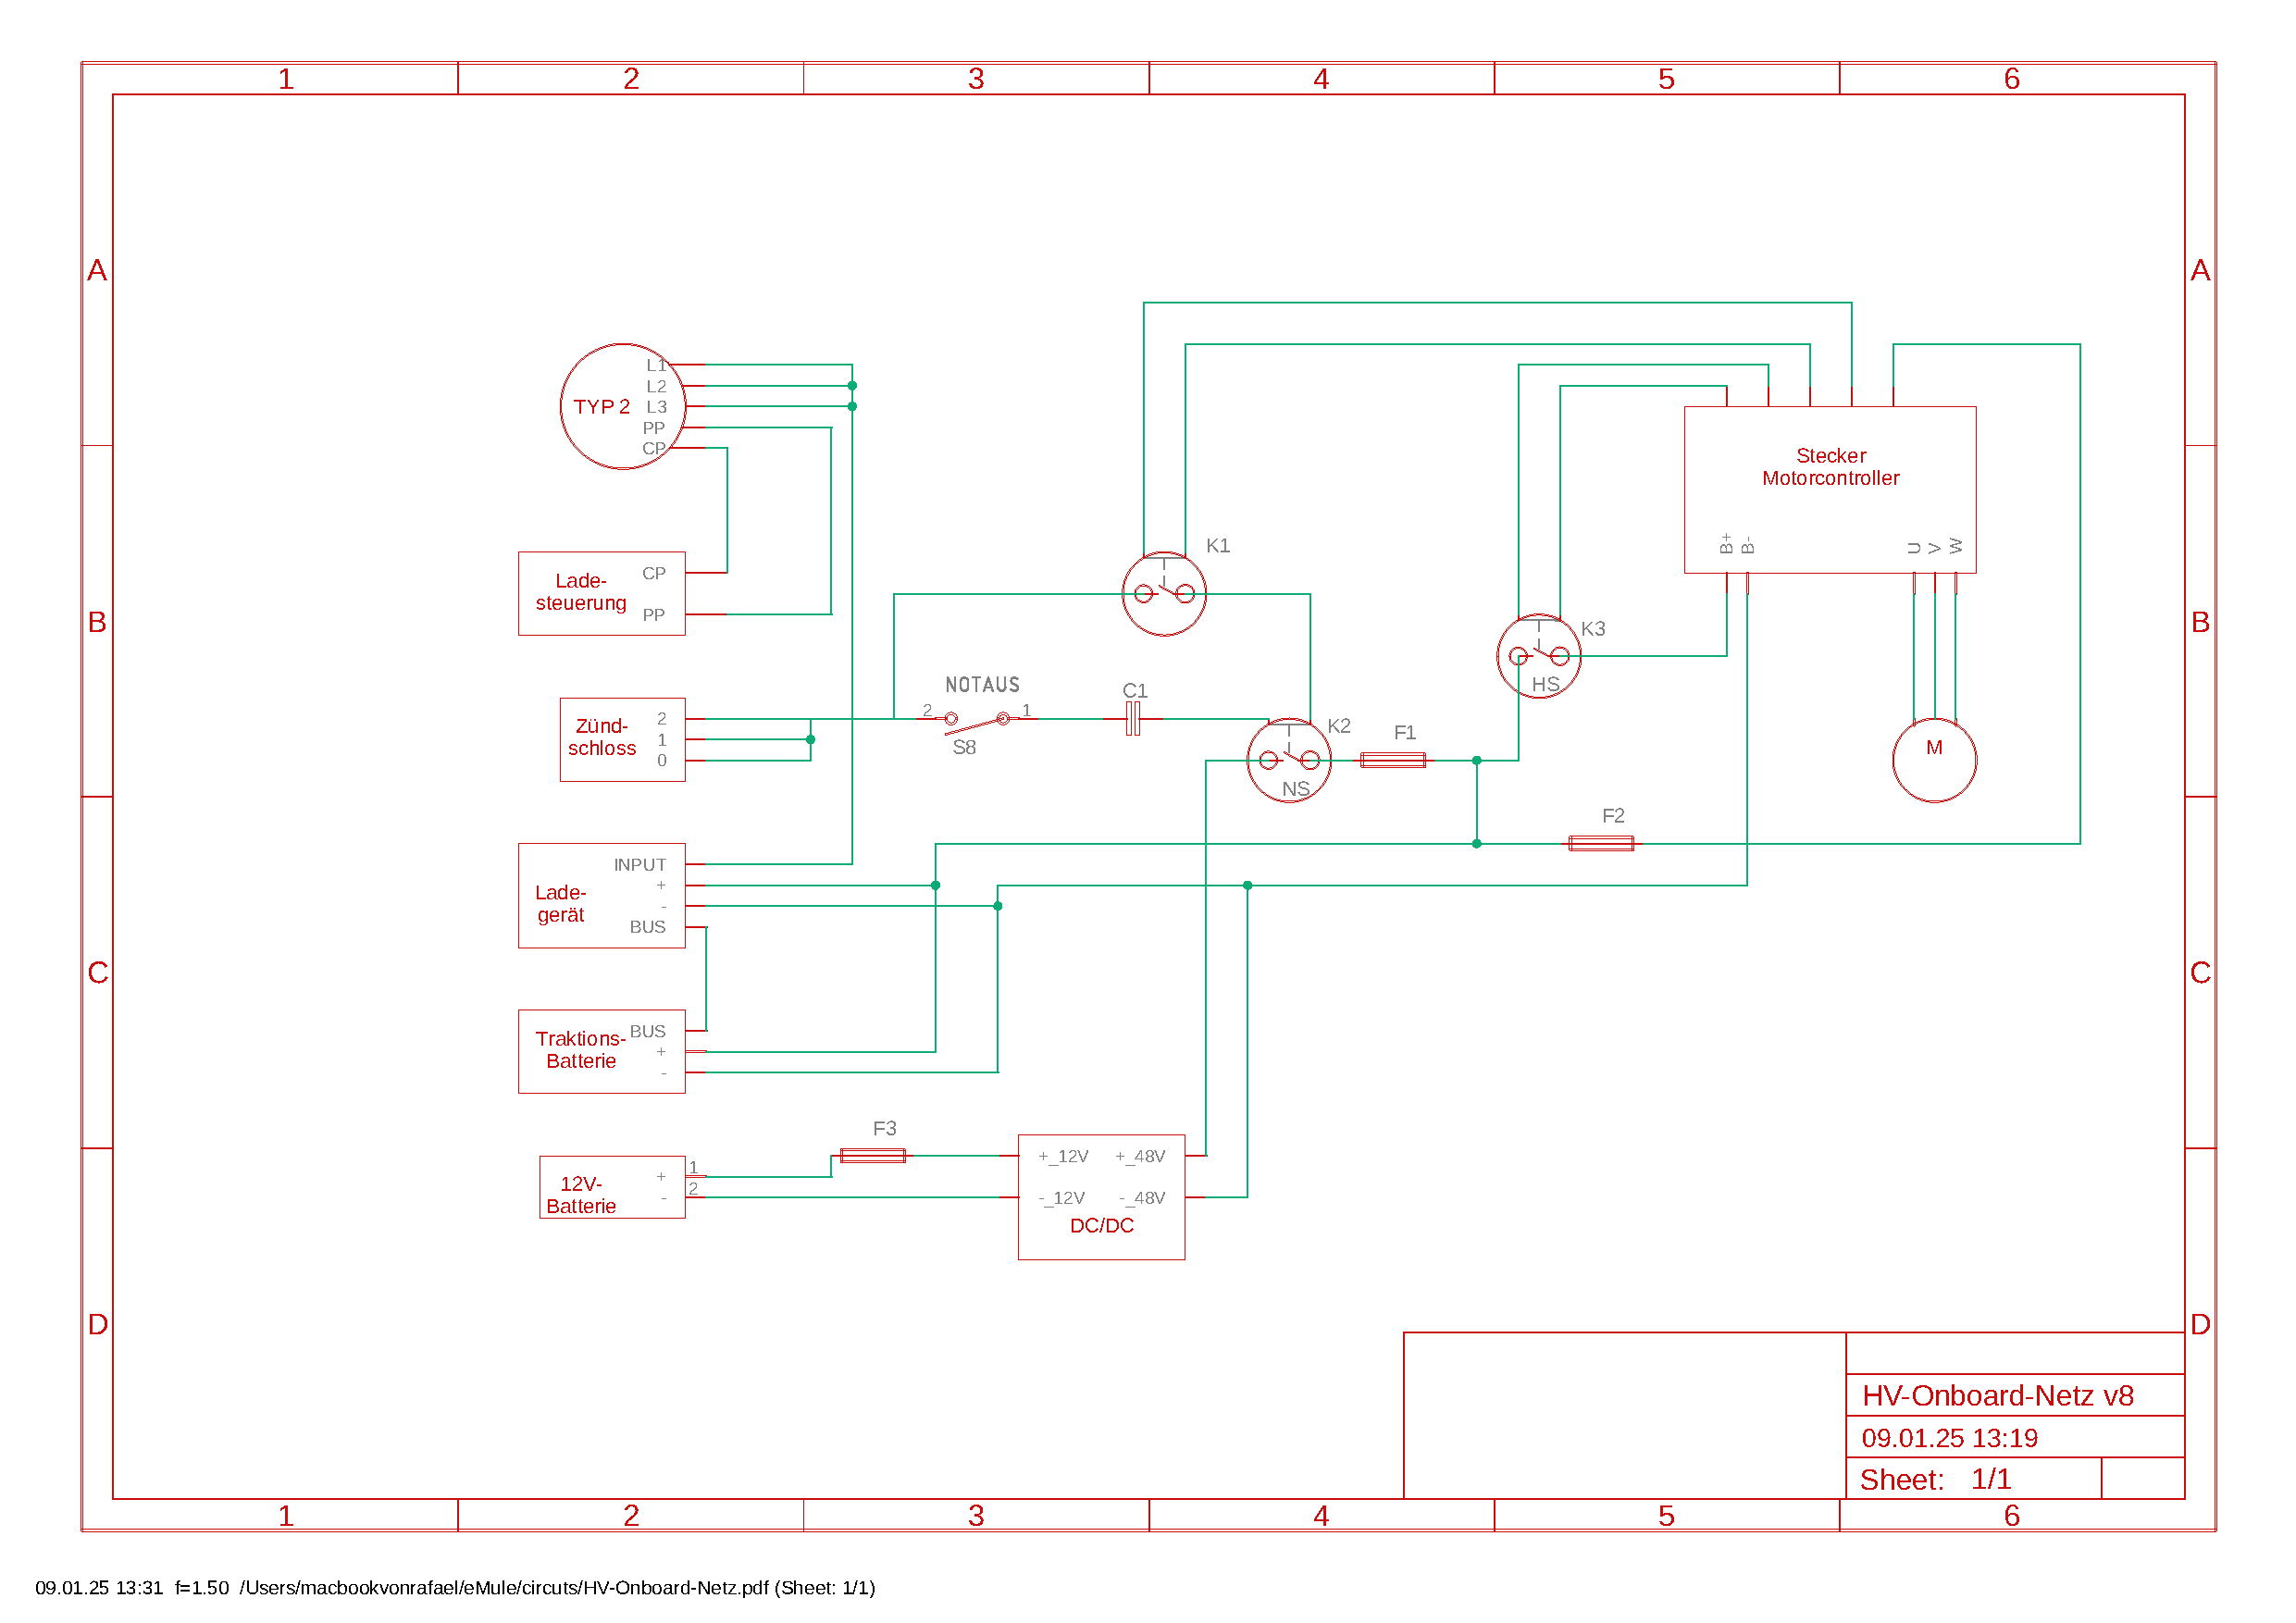
\includepdf[pages=1, fitpaper=true, pagecommand={%
	\thispagestyle{empty} % Entfernt Seitenzahlen und Kopfzeilen
	\begin{center}
		\captionof{figure}{Circut diagram of the HV onboard power supply} % Fügt die Caption ein
		\label{fig:hv_onboard_network} % Für Querverweise
	\end{center}
}]{circuts/HV-Onboard-Netz.pdf}
\addtocounter{page}{1}

\subsection{Circut diagram of the charge connector lock }

%Für die Erstellung des \textit{charge connector lock} (siehe Abbildung \ref{fig:hv_onboard_network}) Stromlaufplans nach festgelegter Norm und aktuellem Verbaustand wird zunächst eine händische Skizze des Systems, durch die für den Einbau zuständigen Kollegen, angefertigt und an das Dokumentationsteam weitergegeben. Im ersten Schritt wird dieser Stromlaufplan systematisch auf Unstimmigkeiten, wie fehlende Verbindungen oder unklare Symbolik, überprüft. Gefundene Fehler werden im nächsten Schritt markiert und anschließend korrigiert, wobei die Einhaltung elektrotechnischer Standards gewährleistet wird. Zudem erfolgt eine Layoutanpassung zur Verbesserung der Übersichtlichkeit. Im letzten Schritt muss die Normkonformität der Stromlaufplanskizze überprüft werden. Der überarbeitete Stromlaufplan wird abschließend mit Autodesk Fusion 360 in ein DIN-A3-Format übertragen. Dabei werden Titelblock und Legende integriert, um die Professionalität und Lesbarkeit sicherzustellen.
In order to create the charge connector lock (see figure \ref{fig:Charge_Connector_Lock_v10}), it is first necessary to create a manual sketch of the system. This is to be done according to the defined standard and current installation status. The creation of the manual sketch is the responsibility of the colleagues who are responsible for installation. It is then to be passed on to the documentation team. In the initial phase, the circuit diagram is meticulously examined for any potential discrepancies, including the absence of connections or the ambiguity of symbols. Any errors detected during this process are subsequently annotated in the subsequent stage, and then rectified, thus ensuring conformity with the relevant electrotechnical standards. The layout has been adapted to improve clarity. In the final step of the process, the conformity of the circuit diagram with the relevant standards must be checked. The revised circuit diagram is then transferred to a DIN A3 format using Autodesk Fusion 360. The integration of the title block and legend is a deliberate design choice that serves to enhance the document's professionalism and legibility.
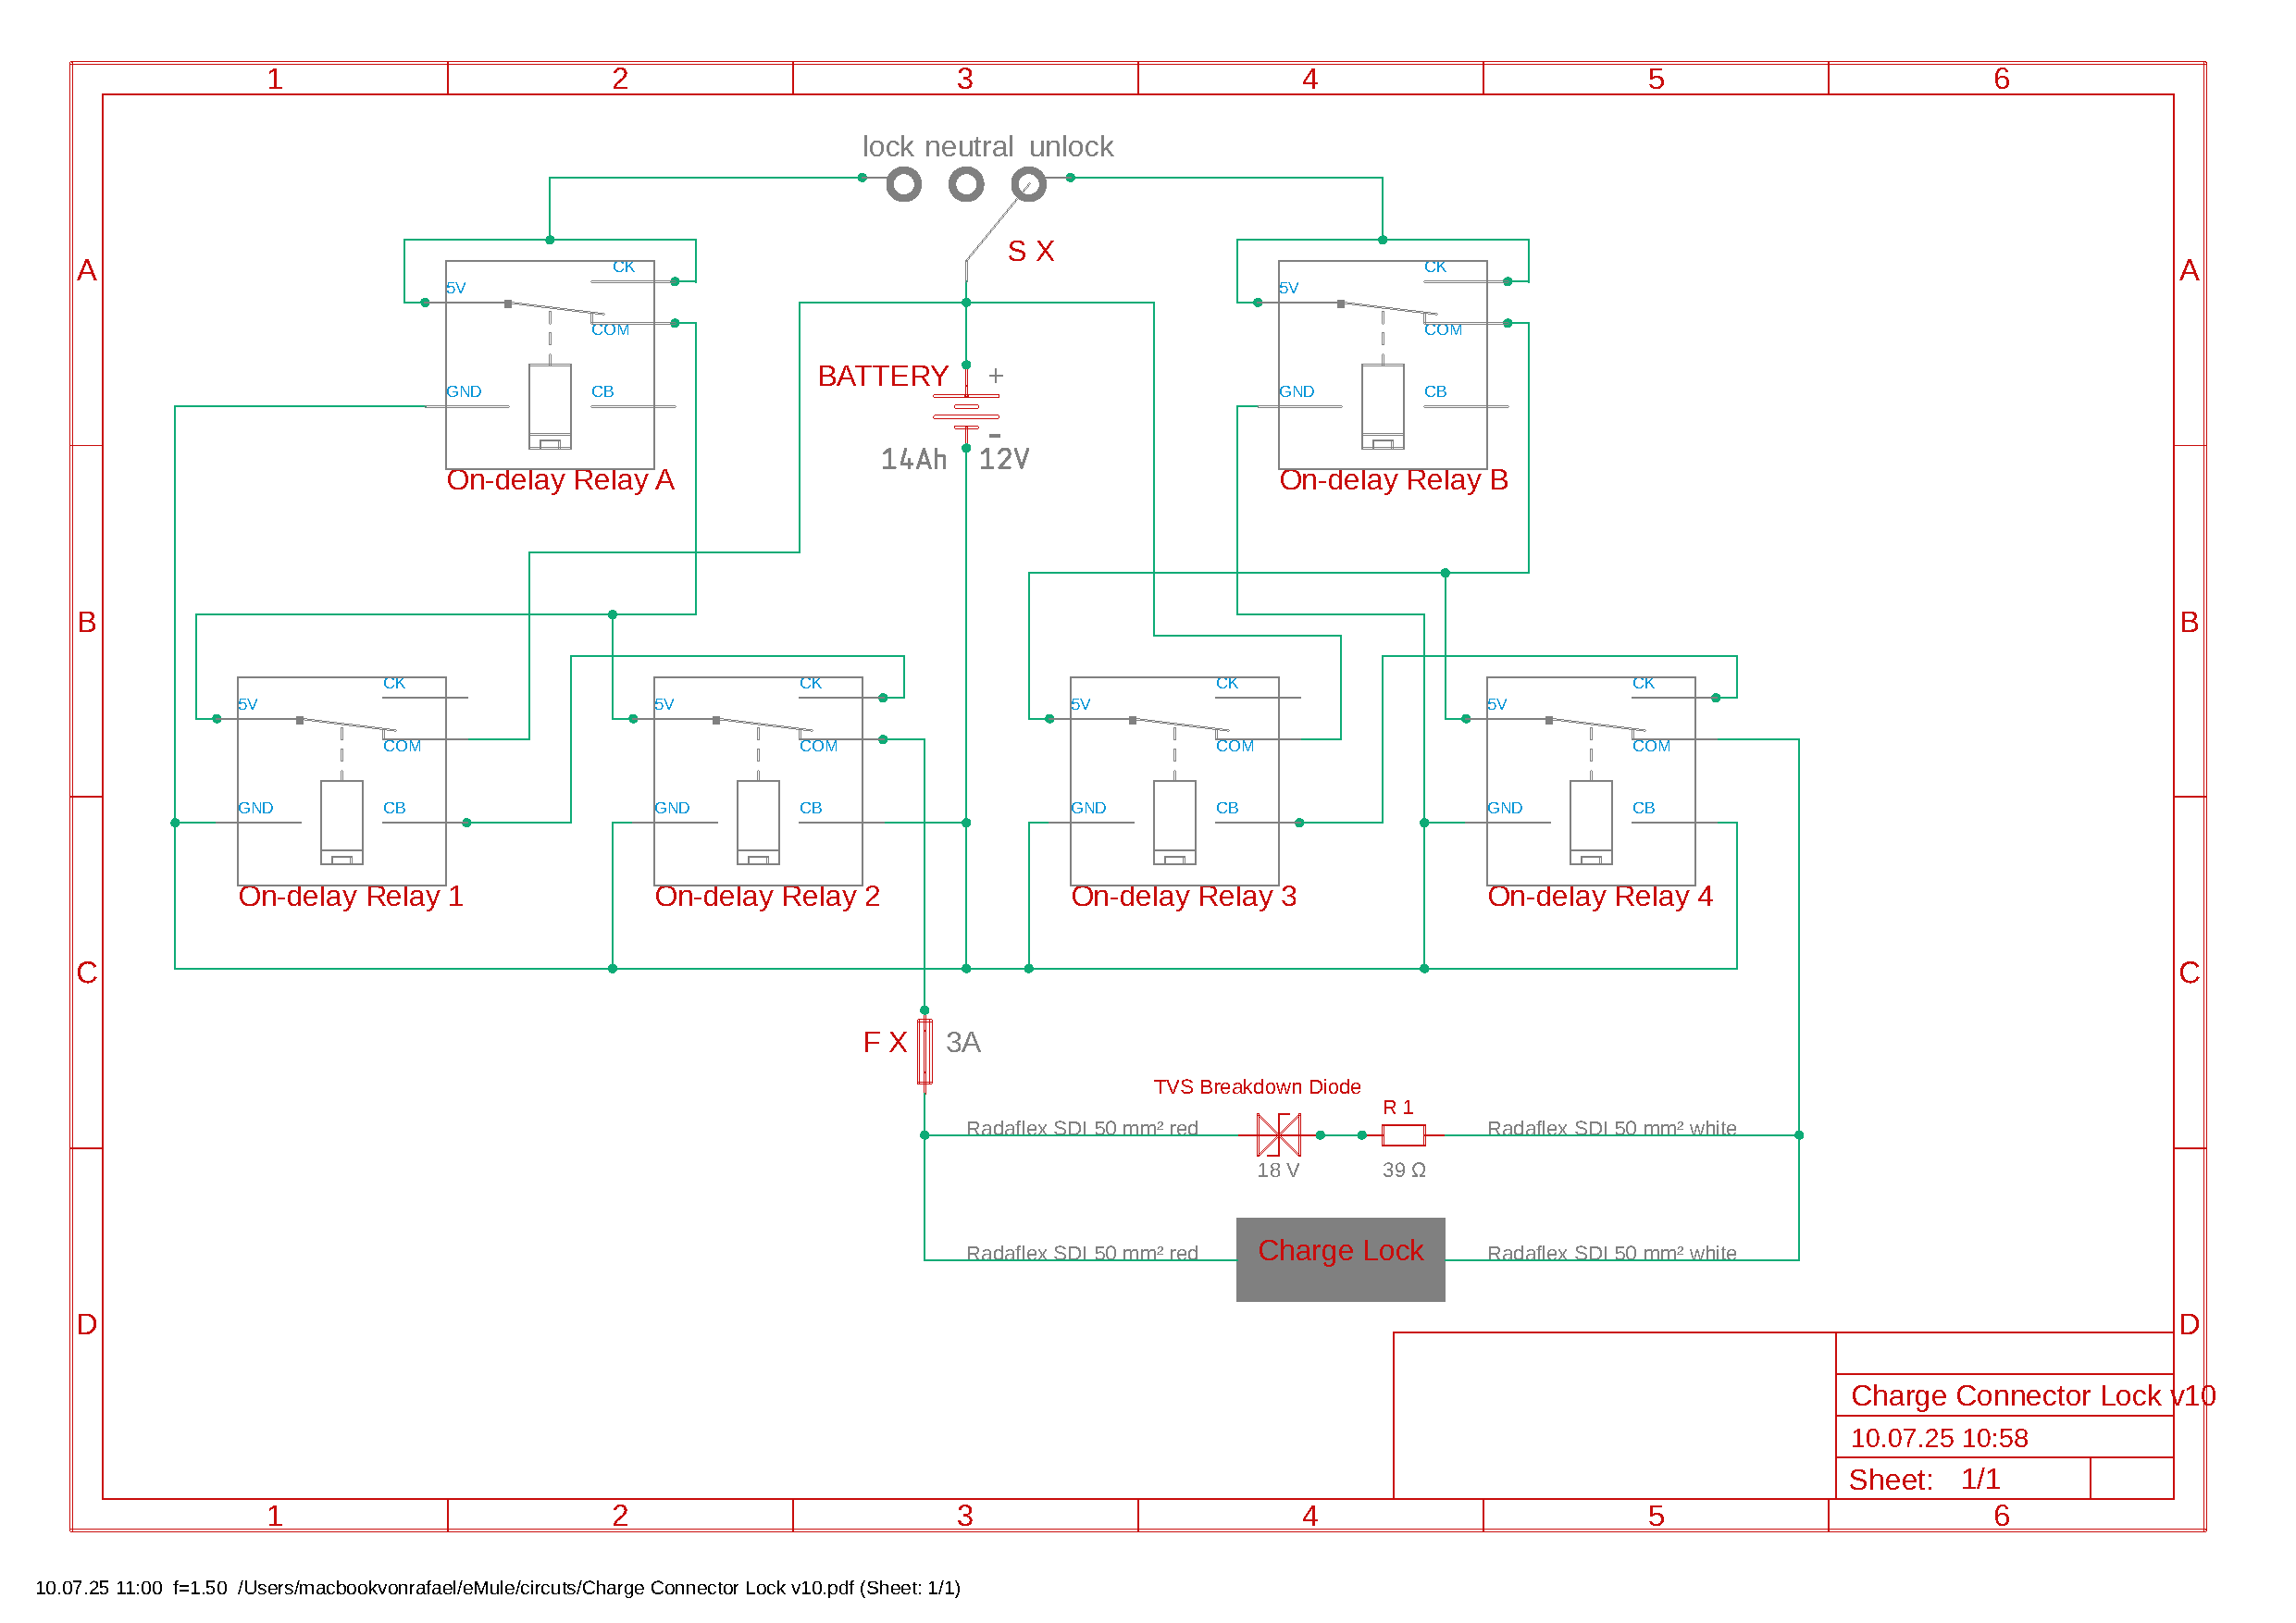
\includepdf[pages=1, fitpaper=true, pagecommand={%
	\thispagestyle{empty} % Entfernt Seitenzahlen und Kopfzeilen
	\begin{center}
		\captionof{figure}{Circut diagram of the charge connector lock} % Fügt die Caption ein
		\label{fig:Charge_Connector_Lock_v10} % Für Querverweise
	\end{center}
}]{circuts/Charge Connector Lock v10.pdf}
\addtocounter{page}{1}

\section{Legende der Schaltzeichen}
%In der folgenden Tabelle (siehe Abbildung \ref{tab:legende}) werden die verwendeten Schaltzeichen des Stromlaufpläne gemäß der Norm DIN EN 60617 erläutert. Diese Schaltzeichen dienen dazu, die elektrischen Komponenten und deren Verbindungen im Stromlaufplan eindeutig und standardisiert darzustellen. Die Legende bietet eine Übersicht über jene Symbole, die in den vorangegangenen Stromlaufplänenplänen verwendet werden, und erleichtert so das Verständnis der Systemarchitektur und Funktionalität der einzelnen Pläne sowie des Gesamtsystems. Dieses Verzeichnis umfasst aktuell:
The subsequent table (see figure \ref{tab:legende}) provides a comprehensive explanation of the circuit symbols employed in the circuit diagrams, in accordance with the DIN EN 60617 standard. These symbols are employed to denote the electrical components and their interconnections in the circuit diagram in a manner that is both clear and standardised. The legend offers a comprehensive overview of the symbols utilised in the preceding circuit diagrams, thereby facilitating comprehension of the system architecture and functionality of the individual diagrams and the overall system. The directory under discussion currently includes:

\begin{multicols}{2}
	\begin{itemize}
%		\item Schütz
%		\item Kondensator
%		\item Funkenstrecke
%		\item Masse
%		\item Batterie
%		\item Sicherung
%		\item Schalter
		\item Contactor
		\item Capacitor
		\item Spark gap
		\item Ground
		\item Battery
		\item Fuse
		\item Switch
	\end{itemize}
	\columnbreak
	\begin{itemize}
%		\item Positive Temperature Coefficient (PTC)-Wiederstand
%		\item Potentiometer
%		\item Stecker
%		\item LED (Light Emitting Diode)
%		\item Spule
%		\item Drei-Phasen-Motor
\item PTC (Positive Temperature Coefficient) resistor
\item Potentiometer
\item Plug
\item LED (Light Emitting Diode)
\item Coil/Inductor
\item Three-phase motor
	\end{itemize}
\end{multicols}

Im weiteren Verlauf des Projekts kann dieses Verzeichnis beliebig um weitere Schaltzeichen ergänzt und angepasst werden.

\begin{table}[h!]
	\centering
	\resizebox{0.75\textwidth}{!}{% Verkleinert die gesamte Tabelle auf 90 % der Textbreite
		\renewcommand{\arraystretch}{1.8}
		\setlength{\tabcolsep}{15pt}
		\begin{tabular}{|m{5cm}|m{7cm}|}
			\hline
			\textbf{Symbol} & \textbf{Beschreibung} \\
			\hline
			\centering\includegraphics[width=2cm]{Legende/Schütz.png} & \centering Contactor \tabularnewline
			\hline
			\centering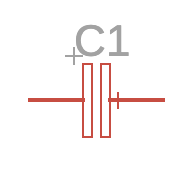
\includegraphics[width=2cm]{Legende/Kondensator.png} & \centering Capacitor \tabularnewline
			\hline
			\centering
\includegraphics[width=2cm]{Legende/Funkenstrecke.png} & \centering Spark gap \tabularnewline
			\hline
			\centering
\includegraphics[width=2cm]{Legende/Ground.png} & \centering Ground \tabularnewline
			\hline
			\centering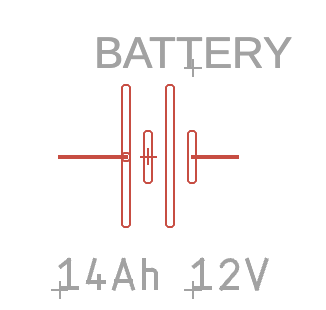
\includegraphics[width=2cm]{Legende/Batterie.png} & \centering Battery \tabularnewline
			\hline
			\centering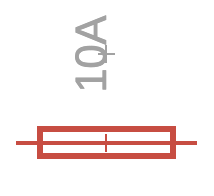
\includegraphics[width=2cm]{Legende/Sicherung.png} & \centering Fuse \tabularnewline
			\hline
			\centering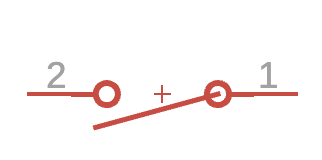
\includegraphics[width=2cm]{Legende/Schalter.png} & \centering switch \tabularnewline
			\hline
			\centering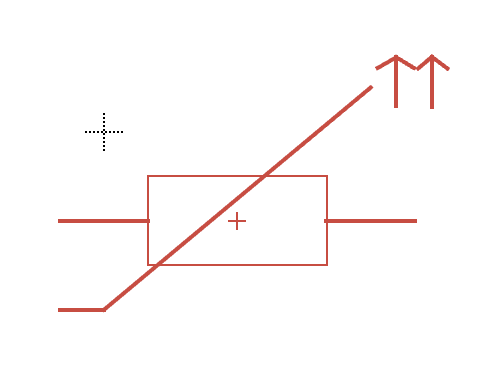
\includegraphics[width=2cm]{Legende/PTC-Widerstand.png} & \centering PTC resistor \tabularnewline
			\hline
			\centering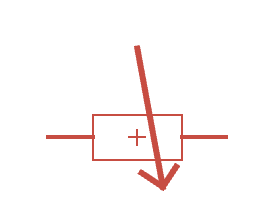
\includegraphics[width=2cm]{Legende/Potentiometer.png} & \centering Potentiometer \tabularnewline
			\hline
			\centering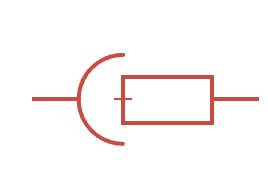
\includegraphics[width=2cm]{Legende/Stecker.png} & \centering Plug \tabularnewline
			\hline
			\centering
\includegraphics[width=2cm]{Legende/LED.png} & \centering LED \tabularnewline
			\hline
			\centering
\includegraphics[width=2cm]{Legende/Spule.png} & \centering Coil/Inductor \tabularnewline
			\hline
			\centering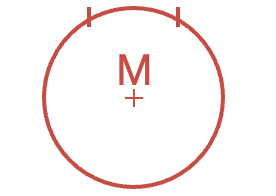
\includegraphics[width=2cm]{Legende/3 Phasen Motor.png} & \centering Three-phase motor \tabularnewline
			\hline
	\end{tabular}}
	\caption{Legende der Symbole}
	\label{tab:legende}
\end{table}
\newpage
\section{Assembly plans}

\subsection{Network assembly plan}
%Die Erstellung des Netzwerkbestückungsplans (siehe Abbildung x) erfolgt gemäß dem aktuellen Verbaustand. Zu diesem Zweck wird der vorliegende Plan zunächst ausgedruckt. Im ersten Schritt erfolgt eine systematische Überprüfung des vorliegenden Stromlaufplans auf Unstimmigkeiten, wie etwa falsche oder fehlende Verbindungen sowie unklare Symbolik. Im darauffolgenden Schritt erfolgt die Markierung der identifizierten Fehler sowie deren Korrektur. Darüber hinaus wird eine Layoutanpassung vorgenommen, um die Übersichtlichkeit zu optimieren. Es ist von essentieller Bedeutung, dass die Komponenten im Plan an der identischen Position wie im Fahrzeug platziert werden. Die Darstellung der relevanten Verbindungen der Bauteile erfolgt in der Planung. Im finalen Schritt wird der überarbeitete Stromlaufplan mit Autodesk Fusion 360 in das DIN-A3-Format übertragen. In diesem Kontext werden Titelblock und Legende integriert, um die Professionalität und Lesbarkeit zu gewährleisten.

The \textit{network assembly plan} (\textbf{see figure \underline{\ref{fig:Network assembly plan}}}) has been formulated in accordance with the current installation status. For the purpose previously outlined, the existing plan is to be printed out. The initial step in this process is to methodically review the existing circuit diagram to identify any inconsistencies, such as erroneous or missing connections, and ambiguous symbols. In the subsequent stage, the errors that have been identified are marked and corrected. Furthermore, the layout has been meticulously revised to enhance clarity. It is imperative that the components are positioned in the same location in the plan as in the vehicle. The relevant component connections are visualised in the planning stage. In the concluding step of the process, the revised circuit diagram is transferred to DIN A3 format using Autodesk Fusion 360. In this particular context, the integration of the title block and legend is paramount to ensure both professionalism and legibility.


\includepdf[pages=1, fitpaper=true, pagecommand={%
	\thispagestyle{empty} % Entfernt Seitenzahlen und Kopfzeilen
	\begin{center}
		\captionof{figure}{Network assembly plan} % Fügt die Caption ein
		\label{fig:Network assembly plan} % Für Querverweise
	\end{center}
}]{circuts/Netzwerkübersicht_eMule.pdf}
\addtocounter{page}{1}

\subsection{Vehicle assembly plan}
%Die Erstellung des Fahrzeugbestückungsplans (\textbf{see figure !!!Buck einfügen!!!!\underline{}}) erfolgt gemäß dem aktuellen Verbaustand. Zu diesem Zweck wird zunächst eine händische Skizze des Systems angefertigt und ausgedruckt. Im ersten Schritt erfolgt eine systematische Überprüfung des vorliegenden Stromlaufplans auf Unstimmigkeiten, wie etwa falsche oder fehlende Verbindungen sowie unklare Symbolik. Im darauffolgenden Schritt erfolgt die Markierung der identifizierten Fehler sowie deren Korrektur. Darüber hinaus wird eine Layoutanpassung vorgenommen, um die Übersichtlichkeit zu optimieren. Es ist von essentieller Bedeutung, dass die Komponenten im Plan an der identischen Position wie im Fahrzeug platziert werden. Die Darstellung der relevanten Verbindungen der Bauteile erfolgt in der Planung. Im finalen Schritt wird der überarbeitete Stromlaufplan mit Autodesk Fusion 360 in das DIN-A3-Format übertragen. In diesem Kontext werden Titelblock und Legende integriert, um die Professionalität und Lesbarkeit zu gewährleisten.
The \textit{vehicle assembly plan} (see figure \ref{fig:Assembly Drawing v7}) has been created according to the current installation status. For the purpose of illustration, a manual sketch of the system is initially created and subsequently printed. The initial step in this process is to methodically review the sketch of the assembly plan to identify any inconsistencies, such as erroneous or missing connections, and ambiguous symbols. In the subsequent stage, the errors that have been identified are marked and corrected. Furthermore, the layout has been meticulously revised to enhance clarity. The components must be placed in the plan with the utmost precision, ensuring that they are positioned identically to their counterparts in the vehicle to ensure optimal functionality. The relevant component connections are visualised during the planning phase. In the concluding step of the process, the revised circuit diagram is transferred to DIN A3 format using Autodesk Fusion 360. In this context, the title block and legend are integrated to ensure both professionalism and legibility.


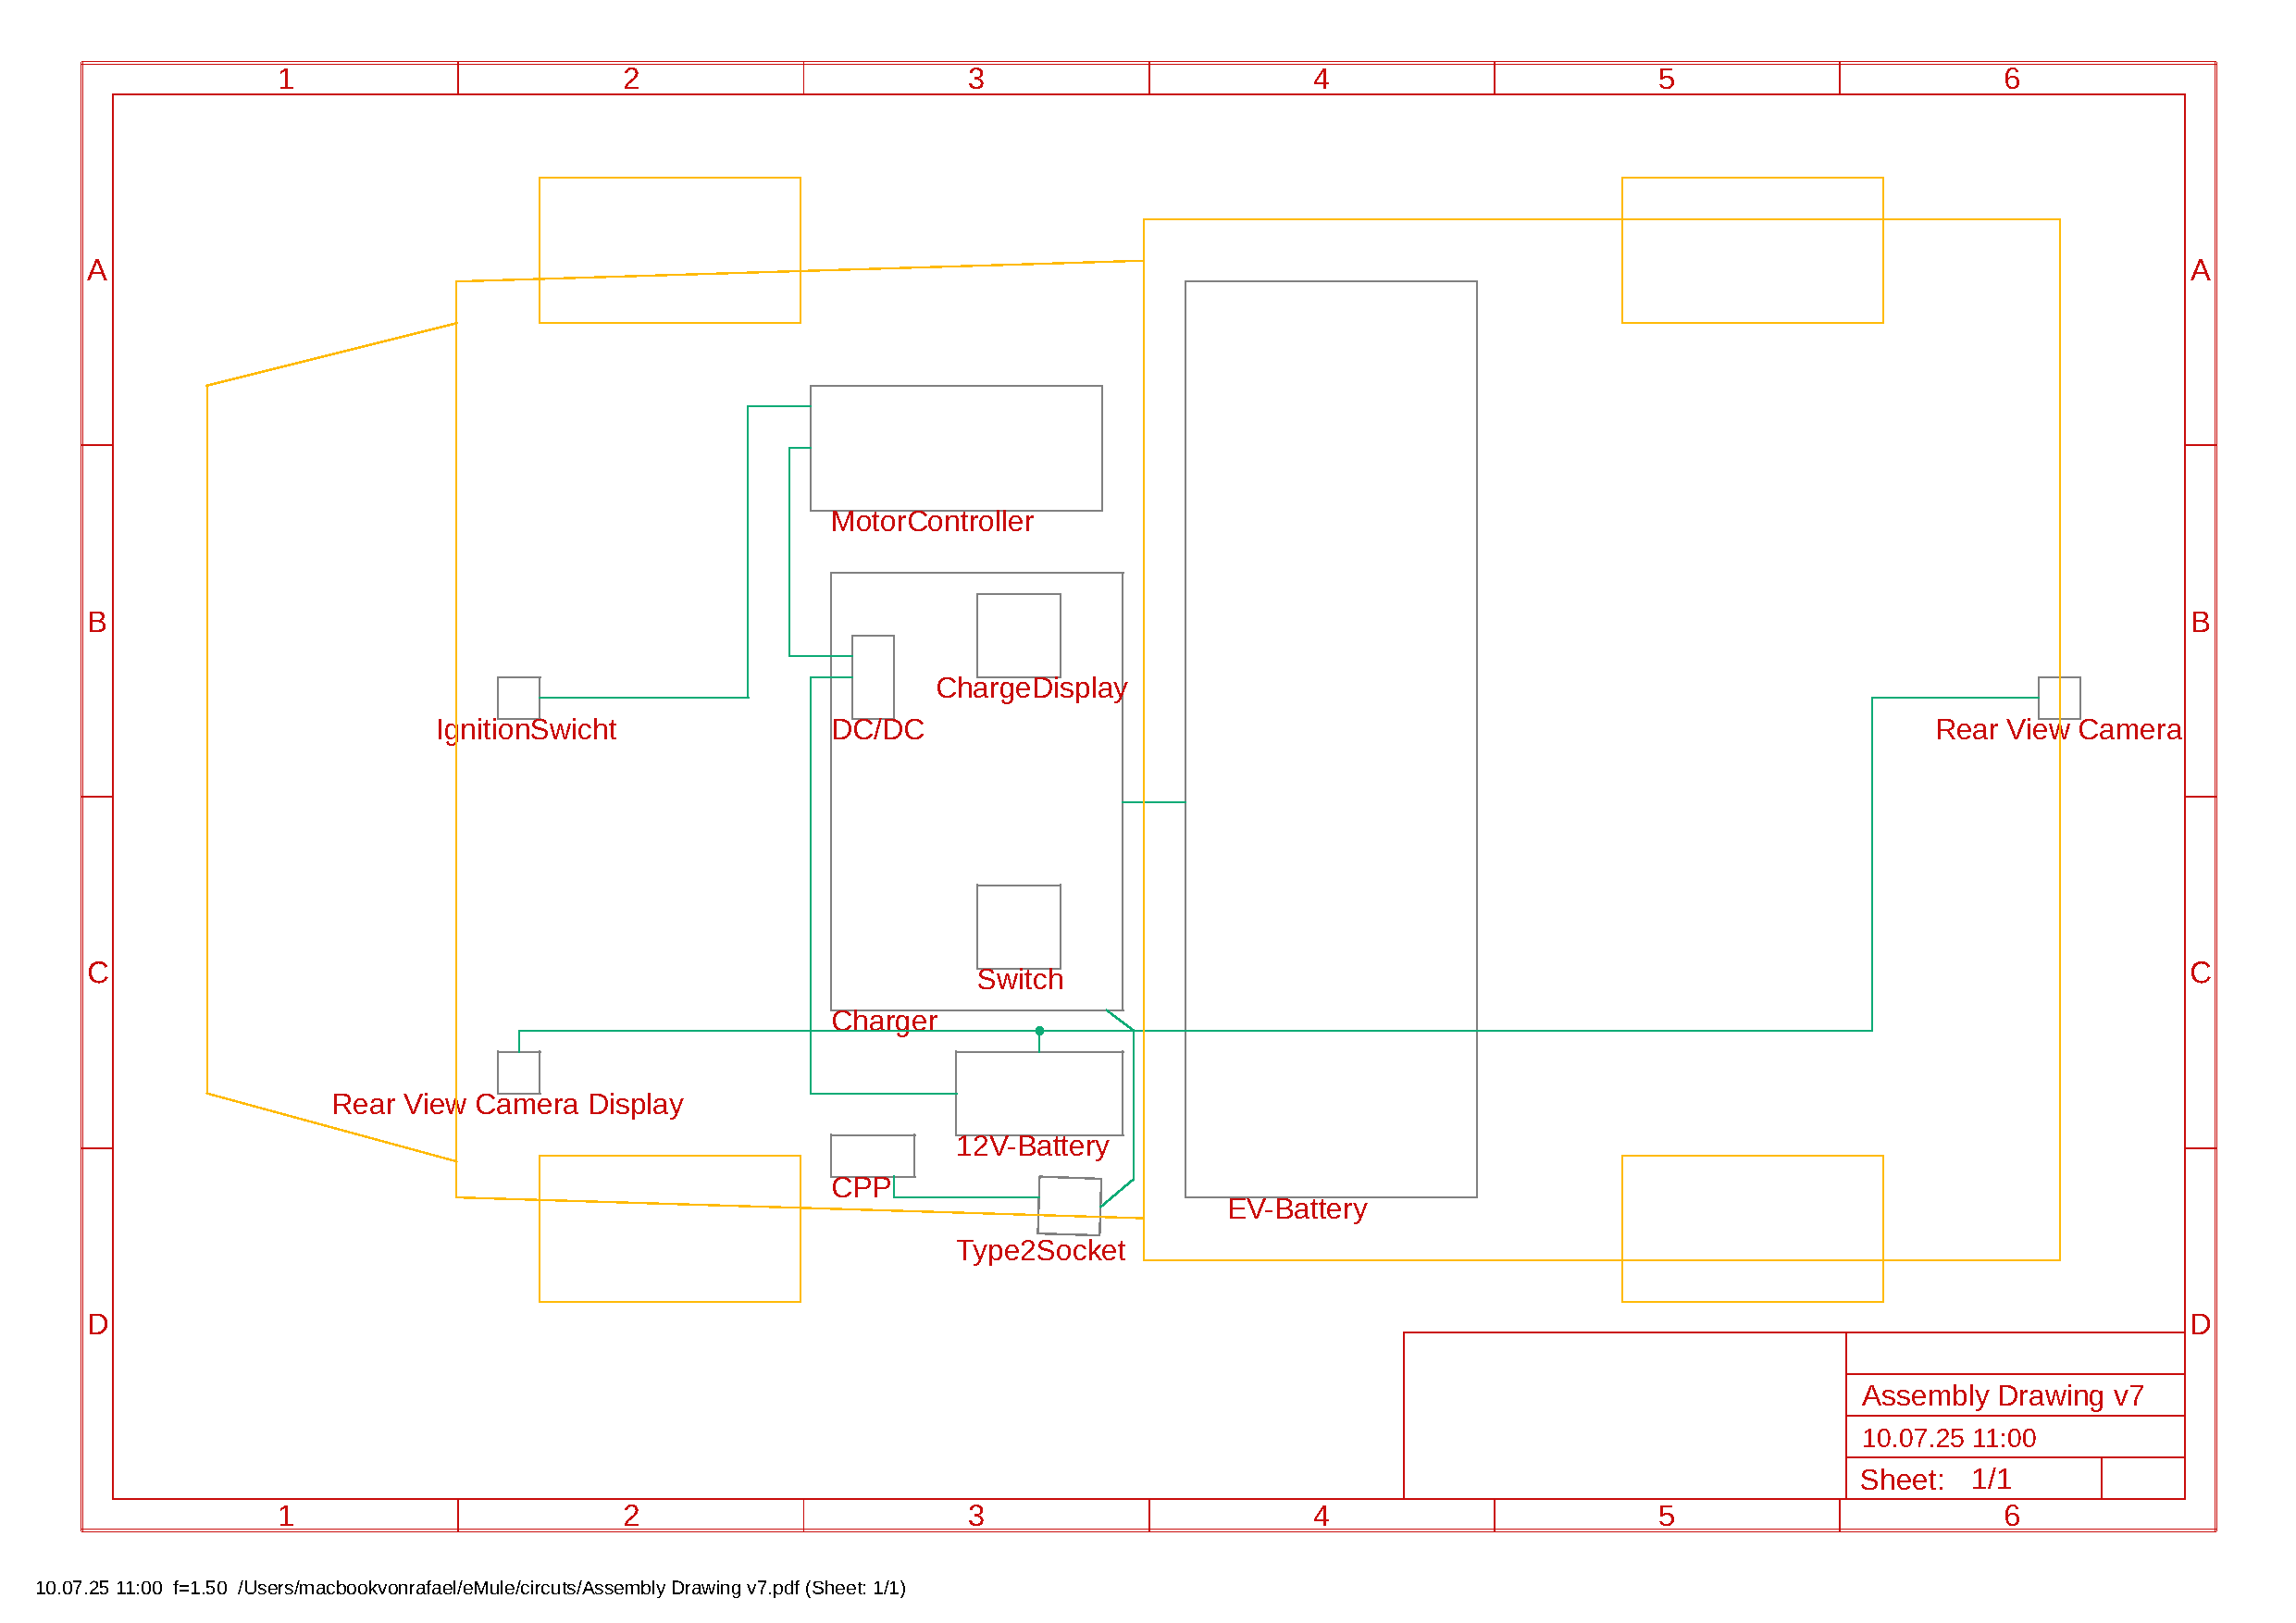
\includepdf[pages=1, fitpaper=true, pagecommand={%
	\thispagestyle{empty} % Entfernt Seitenzahlen und Kopfzeilen
	\begin{center}
		\captionof{figure}{Vehicle assembly plan} % Fügt die Caption ein
		\label{fig:Assembly Drawing v7} % Für Querverweise
	\end{center}
}]{circuts/Assembly Drawing v7.pdf}
\addtocounter{page}{1}